\chapter{Theoretical Description}

This chapter describes the CFT processor from a theoretical
perspective.

For a hardware description of the units described here and more minor ones
beyond the scope of a theoretical discussion, please refer
to~\ccf{chap:processor-hardware-description}. For a description of the
processor's programming model, please refer to~\ccf{chap:programming-model}.


\section{Datapath}

%% \begin{figure}
%% 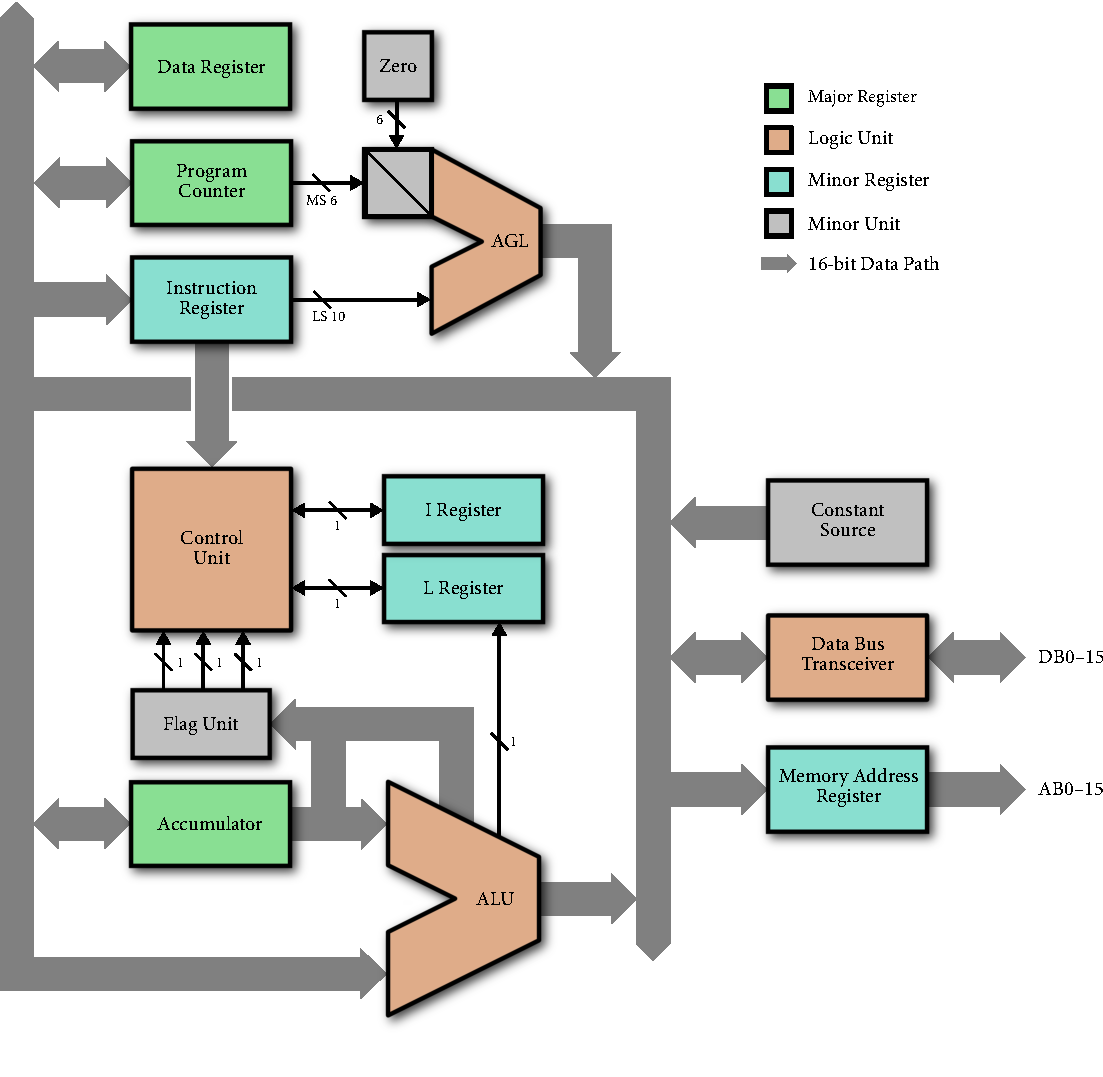
\includegraphics[width=0.95\columnwidth]{figs/datapath2.pdf}\vspace{2em}\\
%% \caption[CFT Datapath]{\label{fig:datapath} The CFT Datapath. }
%% \end{figure}
\begin{figure}
\inputfigure{figure-datapath3}
\caption[CFT Datapath]{\label{fig:datapath} The CFT Datapath. }
\end{figure}

The CFT datapath, illustrated in~\fcf{fig:datapath}, is organised around a
single internal bus, the \IBUS{}. This precludes pipelining techniques, but keeps
the processor easy to reason about and implement. A number of units may either
write to the \IBUS{}, or read from it. The \IBUS{} may also be connected to the
external \DBUS{} via the Data Bus Transceiver, so that data can be exchanged
between the processor and its peripherals.

The Control Unit (centre left) is disjoint from the \IBUS{}, but controls what
other units are connected to it. To do so, it consults the values of registers
and flags.

The \ALU{} is responsible for all high-level operations performed by
the processor. It can perform a number of binary and unary
operations. All operations involve the \gls{Accumulator} (see below). Binary
operations involve the current value of the \gls{Accumulator} and the value
of the \IBUS{}. The \ALU's operations update some of the flags used by
the control Unit.

Ancillary to the \ALU{} is the Constant Store, which can provide a small
number of constant values to the \IBUS{}. These are useful for a number of
operations, such as clearing registers by assigning them the zero constant.

The Flag Unit is illustrated in the datapath as a clearing house for the values
of various flags in the processor. It does not have a corresponding physical
unit, as flags feed directly into various parts of the Control Unit, but it
helps illustrate simply how this is done.

There are three {\em major\/} registers in the datapath: the \gls{Accumulator} (\A),
the Data Register (\DR), and the Program Counter (\PC). Major registers are
16-bits wide. They may be read from or written to, incremented by one, or
decremented by one.

Of these, the \A{} is used as a general-purpose register, permanently and
directly supplying the left operand of the \ALU, and generating flags
used by the Control Unit in decision making.

The \PC{} is used to store the location in memory of the next instruction to be
executed.

The \DR{} is used to store temporarily intermediate addresses used for indirect
memory accesses.

A number of {\em minor registers} are also available. These are either narrower
than 16 bits, or have various restrictions placed on them. The Interrupt
(\Ireg{}) register is a single-bit register that controls whether asynchronous
interrupts may temporarily stop the processor. The {\em Link Register} (\Lreg)
is a versatile single-bit register: it is used as a flag, a carry out bit,
carry in bit, a borrow bit, or a shift register, and is usually treated as a
one-bit extension of the \A{} register. Finally, the \IR{} is a 16-bit
write-only\footnote{It is write-only from the point of view of the \IBUS{} only
  — the Control Unit reads its value continuously.} register permanently
connected to the Control Unit, and controlling its behaviour.

The memory Address Register (\AR{}) is a write-only 16-bit register that stores
an address, and when required, writes this address onto the \ABUS{} to
facilitate external read/write cycles.

Memory addresses used for data are calculating by the \AGL{}, which is
responsible for implementing addressing modes. The \AGL{} can generate 16-bit
addresses either close to the current instruction (by using the top bits of the
\PC{}), or near the beginning of memory (by zeroing the top bits).

\section{Major States}
\label{sec:major-states}

The major states of the processor are fairly conventional, as are the transitions between them:

\begin{description}
\li{Reset.} The initial state of the processor. This state is
  entered asynchronously when computer is reset, and remains in this state for
  a set number of clock periods, according to the operation of the reset
  sequencer. During the reset state, slow units stabilise (after being powered
  on, or after a brown out), and numerous registers in the computer are cleared
  to sane values.
  %the \ns{RESET} line is asserted. The processor remains in this state until
  %the reset state machine deasserts \ns{RSTHOLD}, usually after a hardwired
  %number of clock cycles. In the Reset state, internal state is cleared, and
  %the \PC{} is set to the reset vector (\hex{FFF0}).

\li{Fetch.} In this state, the processor performs a memory read to
  get the contents of the \IR, which implicitly jumps to the appropriate
  microprogram, and to the Execute state. The Fetch state is entered at the end
  of the Reset state; at the end of the Stop state once the computer is no
  longer halted; at the end of the Interrupt state once the interrupt
  microprogram has executed; and at the end of the Execute state, when the
  microprogram signals its end — the Fetch-Execute loop forms the implicit Run
  state. In fact, Fetch and Execute are not explicitly signalled: Fetch is
  simply the first memory read cycle of a microprogram, and Execute is the
  remainder. The distinction is only useful in theory\footnote{And on the front
    panel, which actually includes Fetch and Execute lights, decoded based on
    the value of the Control Unit \register{μPC}.}.

\li{Execute.} In this state, the instruction retrieved in the
  Fetch state is executed. This state is only entered at the end of the Fetch
  state and is where all the processing is carried out. At the end of the
  Execute state, the processor usually re-enters the Fetch state to retrieve
  the next instruction, but may also enter the Interrupt state.

\li{Interrupt.} The Interrupt state is entered at the end of the Execute state
if an interrupt has been previously been signalled and interrupts are
unmasked. In this state, the processor saves certain registers and jumps to a
hardwired location holding an interrupt service routine. The actual workings of
interrupts are slightly more complicated than this, as outlined in
\cf{sec:interrupts-state-machine}.
  %sets the \PC{} to the hardwired interrupt vector (\hex{FFF8}).

\li{Stop.} In this state, the processor's microprogram counter
  (\UPC) is inhibited, freezing the processor. The clocks are still
  running, allowing peripherals that use them to operate. This state is entered
  while the computer is halted. The processor's design is fully static, so it
  may stay in the Stopped state indefinitely.

\end{description}

\section{The Wait State}

The Wait State is a transient, astable state. It may be entered at any time,
though it has special meaning during memory or I/O cycles and is easier to
generate during them. As long as a wait state is signalled, the control unit
protracts its current operation. Wait states are meant to be used with devices
too slow to handle the processor's read or write cycles. They allow most of the
processor to operate at its top speed, slowing down only when communicating
with such devices.


%% The Wait State is a transient state. It may be entered at any time
%% when \ns{WS} is asserted, though it has special meaning during memory
%% or I/O cycles.

%% Once the \ns{WS} signal is deasserted, the processor resumes its
%% previous operation at the next clock tick.

%% \todo{Describe this in detail.}

\begin{figure}
  \centering
  \inputfigure{figure-major-states}
  \caption[CFT Processor Major States]{\label{hard:proc:major-states}CFT Processor Major States:
    Reset (R), Fetch (F), Execute (E), Stop (S), and Interrupt (I).}
\end{figure}


\section{Processor Cycle}

Each processor cycle consists of four stages, T1-T4, each at a 90°
phase difference from the previous one, and each lasting 25\% of the
nominal clock period. With the clock running at 4~MHz, each phase
lasts $250\,\mbox{ns}/4 = 62.5\,\mbox{ns}$.

\begin{description}
\item{\bfseries T1:} the microprogram counter increments, generating a
  new microprogram address. A microcode memory lookup begins.
\item{\bfseries T2:} the microcode memory lookup concludes. With 70\,ns
  ROMs, the second phase must be used to wait for the signals to
  stabilise. As this happens, the decoding unit (which is
  asynchronous) decodes the micro-instruction vector into read enable
  signals and write strobe enable signals for the various units.
\item{\bfseries T3:} one of various things can happen at this point.
  \begin{itemize}
    \item If no data transfer is required by the micro-instruction, the
      processor goes idle.
    \item If a data transfer between internal processor units is
      needed, the unit to be read from drives the \IBUS{} with its data.
    \item If a memory or I/O read is requested, \ns{MEM} or \ns{IO} is
      asserted as appropriate. \ns{R} is also asserted at this
      time. This instructs the memory or peripheral to select chips
      and initiate a read cycle. During this phase, the memory or
      peripheral may signal a \ns{WS} to temporarily delay the onset
      of the next phase.
    \item If a memory or I/O write is requested, \ns{MEM} or \ns{IO}
      is asserted as appropriate. This instructs the memory or
      peripheral to select chips and initiate a write cycle. Data is
      driven onto the \IBUS{}, and the \DBUS{} is connected to the
      \IBUS{} to provide valid data for the external device. During
      this phase, the device may assert \ns{WS} to temporarily delay
      the onset of the next phase.
  \end{itemize}
\item{\bfseries T4:} one of various things can happen at this point.
  \begin{itemize}
  \item If no data transfer is required by the micro-instruction, the
    processor remains idle.
  \item If a data transfer between internal processor units is
    needed, the appropriate write enable signal is asserted at this
    point, and the unit latches data from the \IBUS. This also
    happens for memory or I/O reads.
  \item If a memory or I/O write is requested, \ns{W} is
      asserted. The external device latches or clocks data
      accordingly.
  \end{itemize}
\end{description}

\begin{figure*}
\centering
\inputfigure{figure-processor-cycle}
\caption[Phases of a processor cycle]{\label{fig:processor-cycle} The four phases of a processor cycle. Please note that the fetch and decode stages happen asynchronously, since microcode ROM access times are higher than 25\% of the clock period. The \DBUS{} is never accessed during the first half of the processor cycle, which allows other devices (such as a VDU or DRAM refresh circuitry) to access the bus.}
\end{figure*}

%% \section{Interrupts}

%% \chapter{Hardware Description}
%% \label{chap:processor-hardware-description}


%% The CFT processor is made up of a number of relatively simple units connected
%% in way that causes complex (and in fact, Turing Complete) emergent
%% behaviour. The units are as follows:

%% \begin{description}
%%   \item{\bfseries Clock Generator}. This simple unit generates appropriately
%%     phased clocks from one of three clock sources, and allows stopping the
%%     clock and single-stepping.

%%   \item{\bfseries Reset Sequencer}. Handles reset inputs and performs the reset
%%     sequence.

%%   \item{\bfseries Microcode Sequencer}. The nerve centre of the Control
%%     Unit. Based on a number of inputs and a microcode store, this unit outputs
%%     appropriate control signals to drive the other units in the approproriate
%%     sequence.

%%   \item{\bfseries Unit Decoders}. Decodes microcode sequencer vertical signals
%%     to strobes driving individual units.

%%   \item{\bfseries Skip/Branch Logic}. This unit implements flow control by
%%     signalling the Microcode Sequencer (when it requests this) when a microcode
%%     branch is required. This is also used to perform \gls{machine code}-level
%%     skips.

%%   \item{\bfseries Address Generation Logic}. This unit forms half of the
%%     \glspl{Addressing Mode} of the processor.

%%   \item{\bfseries Instruction Register}. Contains the bit pattern of the
%%     instruction currently being executed. This selects a microprogram for the
%%     Microcode Sequencer to run.

%%   \item{\bfseries Interrupt State Machine}. A state machine that handles
%%     interrupt requests and instructs (when appropriate) the Microcode Sequencer
%%     to jump to the interrupt microprogram.

%%   \item{\bfseries Data Bus Driver and Wait States}. A unit that connects the
%%     processor's internal bus to the external data bus, and also generates write
%%     waveforms. As a bonus, it also handles requested wait states.

%%   \item{\bfseries Address Register}. Is a write-only register that holds the
%%     addresses used to drive the external Address Bus and can drive it as
%%     required.

%%   \item{\bfseries Program Counter}. A major 16-bit register that holds the
%%     address in memory of the next instruction to execute. It supports reading,
%%     writing and increments.

%%   \item{\bfseries Data Register}. A major 16-bit register used to implement
%%     Indirect \glspl{Addressing Mode}. This register supports reading, writing,
%%     increments and decrements.

%%   \item{\bfseries Accumulator}. The single general purpose register of the CFT
%%     architecture. This register supports reading, writing, increments and
%%     decrements, and also calculates the zero and negative flags for the Control
%%     Unit and \gls{ALU}.

%%   \item{\bfseries Autoindex Logic}. This unit helps implement Autoindex mode by
%%     notifying the Microcode Sequencer when the appropriate addresses are used.

%%   \item{\bfseries I/O Device Address Decoder}. To simplify address decoding for
%%     peripherals, this unit decodes the upper eight bits of the I/O address
%%     space and provides appropriate chip select signals on the expansion bus.

%%   \item{\bfseries Link Register}. A complex single-bit register with complex
%%     set, clear and toggle inputs.

%%   \item{\bfseries ALU Operationg Decocder}. Receives signals from the
%%     Control Unit and drives appropriate parts of the \gls{ALU}.

%%   \item{\bfseries ALU Binary B Register}. Implements the right-hand register
%%     for \gls{ALU} binary operations.

%%   \item{\bfseries ALU Binary Y Register}. Implements the output register
%%     for \gls{ALU} binary operations.

%%   \item{\bfseries ALU Binary Table}. Implements the binary operation function
%%     table.

%%   \item{\bfseries ALU Unary Table}. Implements the unary operation function
%%     table.

%%   \item{\bfseries Flag Logic}. Implements the flag registers attached to the
%%     \gls{ALU}.

%%   \item{\bfseries 8 kWord Memory Banking Unit}. A simple banked memory
%%     management unit that allows 21 bits of physical memory to fit the CFT's
%%     16-bit address space.

%% \end{description}

%% \begin{figure*}
%% \includegraphics[width=0.95\textwidth]{figs/Processor-Board-A.png}\vspace{2em}\\
%% \caption[Layout of Processor Board A]{\label{fig:layout-board-a} Layout of Processor Board A.}
%% \end{figure*}
%% \begin{figure*}
%% \includegraphics[width=0.95\textwidth]{figs/Processor-Board-B.png}\vspace{2em}\\
%% \caption[Layout of Processor Board B]{\label{fig:layout-board-b} Layout of Processor Board B.}
%% \end{figure*}
%% \begin{figure*}
%% \includegraphics[width=0.95\textwidth]{figs/Processor-Board-C.png}\vspace{2em}\\
%% \caption[Layout of Processor Board C]{\label{fig:layout-board-c} Layout of Processor Board C.}
%% \end{figure*}

%% This chapter discusses the theory of operation of the actual hardware
%% implementation of the processor. It discusses how the theoretical CFT
%% architecture can be implemented as hardware. It is broken down by
%% processor unit, including the minor ones, and examines each in an
%% isolated fashion.

%% \section{Clock Generator}

%% The original intention is to run the processor at a clock rate of 4~MHz (a
%% clock period of 250~ns). This is output by the clock generator circuitry. There
%% are four clock phases, all at a 50\% duty cycle, each at a 90° phase
%% difference. For each rising clock edge, there is a synchronous, corresponding
%% falling clock edge 90° away, and vice versa. Some of these clock phases are
%% used directly in the processor (or computer) circuitry. Others are combined to
%% create specific timing pulses or strobes.

%% A 4:1 multiplexer selects one of three clock sources: the fast clock
%% (\ps{FASTCLK}, nominally at 16~MHz), a slower demonstration clock named
%% \ps{SLOWCLK} (around 200–250 Hz) and a creeping clock for testing and microcode
%% debugging called \ps{TESTCLK} (around 20–25 Hz). The multiplexer selects among
%% the three clocks with two input signals from the front panel, \ps{FPFAST} and
%% \ps{FPSLOW}. The following function table is implemented:

%% \begin{center}
%%   \zebra
%%   \begin{tabular}{*{4}{>{\textsf\bgroup}c<{\egroup}}l}
%%     %\noalign{\smallskip}\hline\noalign{\smallskip}
%%     %\hline
%%     \ps{FPSLOW} & \ps{FPFAST} & Mux AB & Clock \\
%%     %\noalign{\smallskip}\hline\noalign{\smallskip}
%%     \hline
%%     L & L & \bin{00} & \ps{SLOWCLK} \\
%%     H & L & \bin{10} & \ps{TESTCLK} \\
%%     X & H & \bin{X1} & \ps{FASTCLK} \\
%%     \hline
%%   \end{tabular}
%% \end{center}

%% To provide a sane clock selection when no front panel is connected, \ps{FPFAST}
%% is pulled high and \ps{FPSLOW} is pulled low. This selects the fast clock.

%% \paragraph{Fast Clock}

%% To ensure a stable clock with maximal accuracy, the fast clock was implemented
%% as a single-part, four pin, 16~MHz crystal oscillator. The only additional
%% component to this clock source is a 100~nF bypass capacitor.

%% \paragraph{Slow Clock}

%% There are fewer concerns about the accuracy of the slow clock, and duty cycle
%% is immaterial since clocks are subdivided and only the positive edge is used —
%% as such, only the overall {\em clock period\/} is important. Thus, it was
%% easier and more flexible to implement the slow clock using a 555 timer in its
%% standard astable configuration, as shown in~\fcf{fig:555-astable}.

%% \begin{figure}
%% \centering
%% 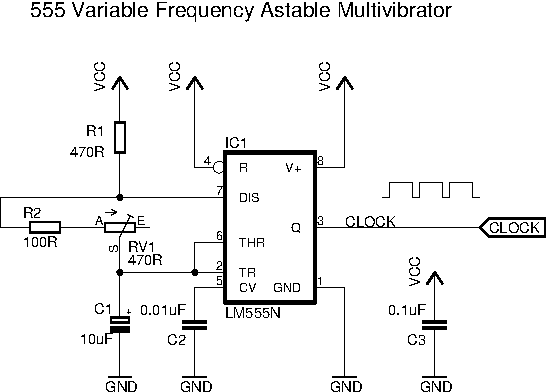
\includegraphics{figs/fig-555-astable.pdf}\\
%% \caption[LM555 in astable configuration] {\label{fig:555-astable}The popular LM555 timer in its astable
%%   configuration, with a variable frequency (and inevitable variable duty
%%   cycle). This one is configured to generate 89–215~Hz frequencies, and is used
%%   as the \ps{SLOWCLK} generator.}
%% \end{figure}

%% \paragraph{Test Clock}

%% The test clock is the same design as the slow clock — in fact, they are both
%% built around the same 556 IC (two 555 timers in one 16-pin \gls{DIP} package).


%%  Each clock source is
%% divided by four internally to generate the four clock phases.

%% \bug{\ps{FPUSTEP} needs to strobe at 2×CLK, this is not very useful.}{} \bug{The slow
%%   clock generators run at ¼ frequency.}{The best way to fix this is to change the 555
%%   capacitor to 2.2µF from 10µF, and adjust the variable resistors.}

%% \todo{Use XOR-based edge detection to generate two pulses (four edges) from one activation
%%   of the \sw{µSTEP} switch.}

%% \todo{Complete this}


%% \begin{figure}
%% \centering
%% \begin{tikztimingtable}
%%   \ns{RAWCLK} & H CL N(A1) 4{CH CL} N(A2) 4{CH CL} N(A3) 4{CH CL} N(A4) 2{CH CL} CH \\
%%   %% \CLOCK{1} (270°)  & L 8H 3{8L 8H} 4L \\
%%   %% \CLOCK{2} (180°)  & 5H 3{8L 8H} 8L \\
%%   %% \CLOCK{3} (90°)   & H 8L 3{8H 8L} 4H \\
%%   %% \CLOCK{4} (0°)    & 5L 3{8H 8L} 8H \\
%%   %% \CLOCK{5}         & L 12H 3{4L 12H} L \\
%%   %% \GUARDPULSE       & 3L ee 3{3H ee 11L ee} 3H ee 8L \\
%%   \CLOCK{1} (0°)       & 3H 3{4L 12H} 4L 6H\\
%%   \CLOCK{2} (90°)      & 7H 3{4L 12H} 4L 2H\\
%%   \CLOCK{3} (180°)     & 11H 3{4L 12H} 2L \\
%%   \CLOCK{4} (270°)     & 3L N(B1) 12H 4L N(B2) 12H 4L N(B3) 12H 4L N(B4) 10H\\
%% %
%%   \extracode
%%   \tablerules
%%   \begin{pgfonlayer}{background}
%%     \foreach \n in {1,...,4}
%%     \draw [help lines] (A\n) -- (B\n);
%%   \end{pgfonlayer}
%% \end{tikztimingtable}
%% \caption{\label{fig:clock-timing} Timing diagram of the four-phase clock generator.}
%% \end{figure}


%% \begin{figure}
%% \centering
%% \begin{tikztimingtable}
%%   \CLOCK{3}    & H CL 4{CH CL} N(A2) 4{CH CL} N(A3) 4{CH CL} N(A4) 2{CH CL} CH \\
%%   \ns{RESET}   & 10H N(A1) 3L ;[dotted] 15L; 7L H ;[dotted] 15H; 10H \\
%%   \ns{RSTHOLD} & 10H 3L ;[dotted] 15L; 8L N(B3) ;[dotted] 15L; 10H \\
%%    \IBUSn{0–15} & 10U{} N(B1) 41D{\hex{FFF0}} N(B4) 10U{} \\
%% %
%%   \extracode
%%   \tablerules
%%   \begin{pgfonlayer}{background}
%%     \foreach \n in {1,4}
%%     \draw [help lines] (A\n) -- (B\n);
%%   \end{pgfonlayer}
%% \end{tikztimingtable}
%% \caption[Reset waveform]{\label{fig:reset-timing} Reset waveform. The width of \ns{RSTHOLD} has
%%   a guaranteed, configurable minimum width and its rising edge is synchronous
%%   to the rising edge of \CLOCK{3}.}
%% \end{figure}


%% \section{Reset Logic}

%% The Reset Logic is a simple 8-bit counter, clocked from the processor clock to
%% ensure the reset pulse is synchronised with the processor sequencer.

%% A number of open drain reset inputs are combined together and fed into the
%% counter's active low reset pin. These include:

%% \begin{itemize}
%% \item The front panel \ns{FPRESET} input. This is connected to a toggle switch
%%   and allows the user to reset the computer manually.
%% \item The power supply \ps{POWEROK} signal. The power supply asserts this when
%%   the power output is healthy. The signal is clear when the power supply is
%%   still stabilising after initial power up, or when a brown-out is
%%   detected. Interpreting it as the imaginary active-low ‘\ns{POWERBAD}’ signal
%%   allows us to reset the machine on brown-outs {\em and\/} to allow for a
%%   power-on reset sequence.
%% \item When the optional reset button on the reset logic board is pressed.
%% \item When the open drain \ns{RESET} signal is asserted. This allows any number
%%   of external drivers of this signal.
%% \end{itemize}

%% When the reset signal goes low, the counter resets and starts counting. A bank
%% of jumpers connects one of the counter's binary outputs to the \ns{RSTHOLD}
%% signal. With the count reset, \ns{RSTHOLD} goes low. When the count progresses
%% enough for the selected bit to go high, \ns{RSTHOLD} goes high
%% (deasserted). This also disables the counter. At this point, the \ns{RSTHOLD}
%% pulse is complete.

%% By selecting which count bit drives \ns{RSTHOLD}, the pulse width can be controlled. In
%% theory, pulse widths of $2^n$ clock periods ($1\leq n\leq 8$) can be used. In practice,
%% because the counter is registered, and the register and count inputs are wired together,
%% the \ns{RSTHOLD} pulse lasts for one extra clock period. Also, since the reset pulse
%% arrives asynchronously, the \ns{RSTHOLD} may be up to one clock period longer yet.

%% With a clock of 4~MHz, the longest reset pulse is 64.25~ms which is fine for most uses:
%% the processor itself is very quick to reset, needing less than one clock period. Other
%% hardware, however, is not as fast. Since a reset sequence also happens when the computer
%% powers up or a brown-out is detected, an extended \ns{RSTHOLD} pulse makes the processor
%% wait for power rail and clock stabilisation (among other potential pitfalls).

%% While \ns{RSTHOLD} is active, the value \hex{FFF0} is driven onto the \IBUS{}
%% using a pair of 74x541 buffers. This is the Reset Vector. The processor uses
%% this value to reset the \PC{} to its initial value.

%% \section{Microprogram Counter}
%% \label{sec:upc}

%% The Microprogram Counter (µPC) is a simple 4-bit counter with reset and dual
%% count enables. A \HC{161} counter was selected for this. The '161 counts on the
%% positive edge of \CLOCK{1}, while the count enables are high. These are driven
%% by \ns{WS} and \ns{HALT}, both pulled up in case the two input signals are
%% physically unconnected.

%% The counter resets to zero when \ns{RSTHOLD} is asserted.

%% The \ns{END} signal and its open drain, external counterpart \ns{ENDEXT} are ANDed
%% together and fed to the '161's active low load signal (\ns{LD}). This loads the counter
%% from the \ps{P1}–\ps{P4} inputs, which are always driven low. This is effectively used to
%% reset the counter when the currently executing microprogram is finished.

%% The counter's output provides the four least significant bits of the microcode address
%% vector, the others being provided by other processor states.

%% The counter implements the following function table:

%% \begin{center}
%%   \zebra
%%   \begin{tabular}{*{6}{>{\textsf\bgroup}c<{\egroup}}l}
%%     %\noalign{\smallskip}\hline\noalign{\smallskip}
%%     %\\\hline
%%     \ps{CLOCK4} & \ns{RSTHOLD} & \ns{END} & \ns{ENDEXT} & \ns{WS} & \ns{HALT} & Function \\
%%     %\noalign{\smallskip}\hline\noalign{\smallskip}
%%     \hline
%%     X   & L & X & X & X & X & Reset counter to 0 asynchronously.\\
%%     \tU & H & L & X & X & X & Reset counter to 0.\\
%%     \tU & H & X & L & X & X & Reset counter to 0.\\
%%     \tU & H & X & X & L & X & Inhibit counting.\\
%%     \tU & H & X & X & X & L & Inhibit counting.\\
%%     \tU & H & H & H & H & H & Increment count (mod 16).\\
%%     \hline
%%   \end{tabular}
%% \end{center}



%% %\tikzset{timing/new counter={char=Q,base=16,reset char=R}}
%% \begin{figure*}
%%   \centering
%% \begin{tikztimingtable}
%%   \CLOCK{4}    & L 2{2H 2L} N(A2) 2H 2L N(A3) 2H 2L N(A4) 2H 2L N(A5) %
%%                  2H 2L N(A6) 2H 2L N(A7) 2H 2L N(A8) %
%%                  2H 2L N(A9) 5{2H 2L} N(A10) 2H 2L N(A11) %
%%                  2H 1 \\
%%   \ns{RSTHOLD} & 2H N(A1) 4L 57H \\
%%   \ns{END}     & 15H 3L 45H \\
%%   \ns{ENDEXT}  & 23Z 3L 37Z \\
%%   \ns{WS}      & 38Z 8L 17Z \\
%%   \ns{HALT}    & 47Z 8L 8Z \\
%%   \UPC         & 2U{} N(B1) 7D{\hex{0}} %
%%                  N(B2) 4D{\hex{1}} %
%%                  N(B3) 4D{\hex{2}} %
%%                  N(B4) 4D{\hex{0}} %
%%                  N(B5) 4D{\hex{1}} %
%%                  N(B6) 4D{\hex{0}} %
%%                  N(B7) 4D{\hex{1}} %
%%                  N(B8) 4D{\hex{3}} %
%%                  N(B9) 20D{\hex{3}} %
%%                  N(B10) 4D{\hex{4}} % 
%%                  N(B11) 2D{\hex{5}} \\
%%   %% \ns{WS} & 20H 3L 54H \\
%%   %% \ns{HALT} & 70H 7L \\
%% \extracode
%%  \tablerules
%%  \begin{pgfonlayer}{background}
%%    \foreach \n in {1,...,11}
%%      \draw [help lines] (A\n) -- (B\n);
%%  \end{pgfonlayer}
%% \end{tikztimingtable}
%% \caption[Microprogram Counter Waveforms]{\label{fig:upc-timing} Timing
%%   diagram of the operation of the microprogram counter (\UPC). The
%%   counter resets synchronously while \ns{RSTHOLD} is asserted. The
%%   rising edge of \CLOCK{4} clears it if either \ns{END} or \ns{ENDEXT}
%%   are asserted, and counting is inhibited when \ns{WS} or \ns{HALT}
%%   are asserted.}
%% \end{figure*}

%% \begin{figure}[tb]
%%   \centering
%%   % -*- latex -*-
\documentclass[border=200pt,class=memoir,preview]{standalone}
% -*- latex -*-

%%%%%%%%%%%%%%%%%%%%%%%%%%%%%%%%%%%%%%%%%%%%%%%%%%%%%%%%%%%%%%%%%%%%%%%%%%%%%%%
%%
%% PACKAGES
%%
%%%%%%%%%%%%%%%%%%%%%%%%%%%%%%%%%%%%%%%%%%%%%%%%%%%%%%%%%%%%%%%%%%%%%%%%%%%%%%%

\usepackage{ifxetex}
\usepackage{graphicx}

\usepackage{verbatim}
\usepackage{ifthen}
\usepackage{float}
\usepackage{floatflt}
\usepackage{lipsum}
\usepackage{layout}
\usepackage{calc}
\usepackage{rotating}
\usepackage{array}
\usepackage{color}
\usepackage[table]{xcolor}
\usepackage[includefoot]{geometry}

% Conditional packages
\ifxetex
  % Load fontspec and set fonts
  \usepackage{fontspec}
  \setmainfont{Minion Pro}
  \setsansfont{Myriad Pro}
  \setmonofont[]{Inconsolata}

  \usepackage{pdftricks}
  \usepackage{pdfpages}

  \def\HCode#1{}

\else
  \newcounter{Hfootnote}
  \newcommand\fontspec[1]{}
  %\usepackage[main=english,greek]{babel}
  \usepackage[utf8]{inputenc}
  \usepackage{newunicodechar}
  \newunicodechar{®}{\HCode{&reg;}}
  \newunicodechar{µ}{\HCode{&mu;}} % ‘micro’ (from latin-1 plane)
  \newunicodechar{μ}{\HCode{&mu;}} % mu (from Greek plane)
  \newunicodechar{–}{--}
  \newunicodechar{—}{---}
  \newunicodechar{×}{\ensuremath{\times}}
  \newunicodechar{°}{\HCode{&deg;}}
  \newunicodechar{±}{\HCode{&plusm;}}
  \newunicodechar{Ω}{\ensuremath{\Omega}}
  \newunicodechar{÷}{\ensuremath{\div}}
  %\newunicodechar{²}{\HCode{&sup2;}}
  \newunicodechar{²}{*2*}
  \newunicodechar{¼}{\HCode{&\#188;}}
  \newunicodechar{½}{\HCode{&\#189;}}
  \newunicodechar{≤}{\HCode{ &le; }}
  \newunicodechar{≥}{\HCode{ &ge; }}
  \newunicodechar{≠}{\HCode{ &ne; }}
\fi

%%%%%%%%%%%%%%%%%%%%%%%%%%%%%%%%%%%%%%%%%%%%%%%%%%%%%%%%%%%%%%%%%%%%%%%%%%%%%%%
%%
%% TABLES
%%
%%%%%%%%%%%%%%%%%%%%%%%%%%%%%%%%%%%%%%%%%%%%%%%%%%%%%%%%%%%%%%%%%%%%%%%%%%%%%%%

\renewcommand*\arraystretch{1.25}
\newcolumntype{P}[1]{>{\raggedright\arraybackslash}p{#1}}


%%%%%%%%%%%%%%%%%%%%%%%%%%%%%%%%%%%%%%%%%%%%%%%%%%%%%%%%%%%%%%%%%%%%%%%%%%%%%%%
%%
%% FIGURE DRAWING WITH PGF/TIKZ
%%
%%%%%%%%%%%%%%%%%%%%%%%%%%%%%%%%%%%%%%%%%%%%%%%%%%%%%%%%%%%%%%%%%%%%%%%%%%%%%%%

\ifxetex
  \usepackage{pgf}
  \usepackage{tikz}
  \usepackage{rotating}
  \usepackage[absolute]{textpos}

  %\usetikzlibrary{arrows,positioning,automata,shadows,fit,shapes,counters}
  \usetikzlibrary{arrows,positioning,automata,shadows,fit,shapes,patterns}
  \usetikzlibrary{shadows.blur}
  %\usetikzlibrary{external}
  %\tikzexternalize[prefix=tikz/]
  %\tikzset{external/system call={xelatex \tikzexternalcheckshellescape -halt-on-error -interaction=batchmode -jobname "\image" "\texsource"}}
  \usepackage{standalone}

  \usepackage{tikz-timing}[2009/07/28]
  \usetikztiminglibrary{either}[2009/07/28]
  \tikzset{>=latex}
  \tikzset{timing/z/.append style={black},}
  \tikzset{timing/.append style={x=1ex, y=2ex, line cap=round, line join=round, line width=1.3pt}}
  \tikzset{timing/slope=0.33}
  \tikzstyle{semithick}=[line width=1pt]
  \tikzstyle{heavy}=[line width=2pt]
  \tikzstyle{heavy outline}=[line width=3.5pt]
  \tikzstyle{plot line}=[line width=4pt]
  \tikzstyle{arrow}=[semithick]
  \tikzstyle{thick arrow}=[heavy]
  \tikzstyle{thick outline arrow}=[thick arrow, heavy outline, color=white, draw opacity=0.8]
  \tikzstyle{help lines}=[dotted, line width=0.5pt]
  \tikzstyle{col1}=[draw=p1,fill=p1!60]
  \tikzstyle{col2}=[draw=p2,fill=p2!60]
  \tikzstyle{col3}=[draw=p3,fill=p3!60]
  \tikzstyle{col4}=[draw=p4,fill=p4!60]
  \tikzstyle{col5}=[draw=p5,fill=p5!60]
  \tikzstyle{col6}=[draw=p6,fill=p6!60]
  \tikzstyle{dropshadow}=[] % shade,blur shadow={shadow blur steps=5, shadow blur extra rounding=1.3pt}]
  \tikzset{fsmstate/.style={state,rectangle,rounded corners,dropshadow,minimum width=10em,line width=1pt}}
  % Create a hatch pattern
  \newlength{\hatchspread}
  \newlength{\hatchthickness}
  % declaring the keys in tikz
  \tikzset{hatchspread/.code={\setlength{\hatchspread}{#1}},
           hatchthickness/.code={\setlength{\hatchthickness}{#1}}}
  \tikzset{hatchspread=3pt,
           hatchthickness=0.4pt}
  \pgfdeclarepatternformonly[\hatchspread,\hatchthickness]% variables
     {hatch}% name
     {\pgfqpoint{-2\hatchthickness}{-2\hatchthickness}}% lower left corner
     {\pgfqpoint{\dimexpr\hatchspread+2\hatchthickness}{\dimexpr\hatchspread+2\hatchthickness}}% upper right corner
     {\pgfqpoint{\hatchspread}{\hatchspread}}% tile size
     {% shape description
      \pgfsetlinewidth{\hatchthickness}
      \pgfpathmoveto{\pgfqpoint{0pt}{\hatchspread}}
      \pgfpathlineto{\pgfqpoint{\dimexpr\hatchspread+0.15pt}{-0.15pt}}
      \pgfusepath{stroke}
     }
\fi


%%%%%%%%%%%%%%%%%%%%%%%%%%%%%%%%%%%%%%%%%%%%%%%%%%%%%%%%%%%%%%%%%%%%%%%%%%%%%%%
%%
%% HYPERREF
%%
%%%%%%%%%%%%%%%%%%%%%%%%%%%%%%%%%%%%%%%%%%%%%%%%%%%%%%%%%%%%%%%%%%%%%%%%%%%%%%%

\makeatletter
\@ifpackageloaded{standalone}{}{
  \ifxetex
    \usepackage[CJKbookmarks,bookmarks=true,bookmarksopen=true,pdfpagelabels,pdfstartpage=1]{hyperref}
  \else
    \usepackage[tex4ht]{hyperref}
  \fi
}

\let\old@part\part
\renewcommand\part[1]{%
  \setcounter{chapter}{0}%
  \old@part{#1}%
}
%\renewcommand*{\theHchapter}{\thepart.\thechapter}
\makeatother


%%%%%%%%%%%%%%%%%%%%%%%%%%%%%%%%%%%%%%%%%%%%%%%%%%%%%%%%%%%%%%%%%%%%%%%%%%%%%%%
%%
%% INDEX AND GLOSSARY
%%
%%%%%%%%%%%%%%%%%%%%%%%%%%%%%%%%%%%%%%%%%%%%%%%%%%%%%%%%%%%%%%%%%%%%%%%%%%%%%%%

\usepackage{makeidx}
% Glossaries
\usepackage[acronym]{glossaries}
%\makeindex
%\makeglossaries
% -*- latex -*-

\renewcommand\glspostdescription{}

\newcommand\newglossaryabbr[3]{%
  \newglossaryentry{abbr#1}{name=\glslink{#1}{#2}, text={#2}, description={#3}}
  \newacronym[description={\glslink{abbr#1}{#2}}]{#1}{#1}{#2}
}

\newglossaryentry{IBUS}{name=IBUS,
  description={
  Internal Bus: the single, internal 16-bit bus of the CFT processor.
  }}
  
\newglossaryentry{Data Bus}{name=Data Bus, description={ A
    16-bit bus used to move data between the processor and
    peripherals.  }}
  
\newglossaryentry{Address Bus}{name=Address Bus, description={A
    16-bit bus used to select a peripheral nor memory location to
    access.}}
  
\newglossaryentry{Video Display Unit}{name=Video Display Unit,
  description={ Video Display Unit (VDU): a device that drives a
    display monitor to show character or graphics data on a
    screen. Often also contains one or more input devices (keyboard,
    mouse).}}
  
\newglossaryentry{von Neumann architecture}{name=Von Neumann architecture,
  description={ Named after the work of
    John von Neumann, the von Neumann architecture is a ‘modern’
    computer architecture that includes a register file, arithmetic
    and logic units, memory and input/output, and uses the same
    storage for programs and data.}}

\newglossaryentry{stored program computer}{name=Stored program computer,
  description={ A type of computer that
    uses the same storage for programs and data. All modern computers
    are stored program computers, allowing self-modification of their
    programs. Early designs and many modern microcontrollers stored
    programs and data in separate media, and did not or could not
    treat programs as data.}}

\newglossaryabbr{ALU}{Arithmetic/Logic Unit}{Describe this!}
\newglossaryabbr{ISR}{Interrupt Service Routine}{Describe this!}
\newglossaryentry{UART}{name=UART, description={
    Short for Universal Asynchronous Receiver/Transmitter. UARTs are
    devices that handle asynchronous serial communications such as RS-232, RS-485 or USB.
    }
}
%% \newglossaryentry{alu}{name=\glslink{ALU}{Arithmetic/Logic Unit}, text=Arithmetic/Logic Unit,
%%   description={TODO}}
%% \newacronym[description={\glslink{alu}{Arithmetic/Logic Unit}}]{ALU}{ALU}{Arithmetic/Logic Unit}

\newacronym{SBU}{SBU}{Skip/Branch Unit}

\newacronym{AGL}{AGL}{Address Generation Logic}

\newglossaryentry{DEB}{name=DEB, description={
    Designation of the CFT Debugging/Testing board, a peripheral that
    allows remote control and testing of the computer and its
    peripherals in the style of a virtual front panel. The DEB board
    is discussed in~\ccf{chap:deb}.
}}

\newglossaryentry{VDU}{name=VDU, description={ Video Display
    Unit. Designation of the CFT graphic card and keyboard
    controller. The VDU board is discussed in~\ccf{chap:vdu}.  }}

\newglossaryentry{MSB}{name=MSB, description={
    Most Significant Bits. Usually used to refer to the upper eight bits of a CFT word.
}}
\newglossaryentry{LSB}{name=LSB, description={
    Least Significant Bits. Usually used to refer to the lower eight bits of a CFT word.
}}

\newglossaryentry{NYBBLE}{name=Nybble, description={Sometimes
    nibble. A four-bit quantity, represented as a single hexadecimal
    digit.
}}

% \newacronym{MCU}{MCU}{Micro-Controller Unit}

\newglossaryabbr{MCU}{Micro-Controller Unit}{A single-chip device
  containing a simple microprocessor, general purpose input/output,
  serial input/output, timers, and other useful devices.}

\newacronym{USB}{USB}{Universal Serial Bus}

\newacronym{GPIO}{GPIO}{General-Purpose Input/Output}

\newglossaryentry{Verilog}{name=Verilog,
  description={
    One of the two major hardware
    description languages, the other being VHDL. In the CFT project,
    Verilog is used to perform 74xxx chip-level simulation and
    verification of the CFT processor.
}}

\newglossaryentry{I2C}{name=I²C, description={A two-wire, open-drain
    bus, often used for communication between \gls{MCU}s and
    peripheral chips, including EEPROMs and sensors. For more
    information, please consult
    \url{http://en.wikipedia.org/wiki/I2C}.}}

\newglossaryentry{data stack}{name=Data Stack,
  description=To Do}

\newglossaryentry{postfix}{name=postfix,
  description=To Do}

\newglossaryentry{stack effect comment}{name=stack effect comment,
  description=To Do}

\newglossaryentry{Wait State}{name=Wait State, 
  description={An additional state added to the processor state machine
  to accommodate slow devices. External devices signal their need for a
  wait state to the processor using an appropriate procotol. The
  processor then enters the Wait State and does not leave until the
  device is ready. The processor performs no action during this time,
  hence the name.}}


\newglossaryentry{Twos Complement}{name=Two's Complement,
  description={Currently the most popular means of representing signed
    integers in binary. For a bit width $n$, non-negative numbers $0 \leq
    x < 2^{n-1}$ are represented as unsigned $n$-bit binary
    integers. Negative numbers $-2^{n-1} \leq x < 0$ are represented in
    the form $2^n - x$, with the most significant bit set. On the CFT,
    with $n=16$, this provides a signed range of $[-32,768,
      32,767]$. Two's complement has many useful mathematical
    properties: only one representation of zero, the most significant
    bit also acts as a sign bit, and both addition and subtraction can
    be performed by the same circuitry. For a full discussion, please refer
    to \url{http://en.wikipedia.org/wiki/Two's\_complement}.  }}

\newglossaryentry{Assembly}{name=Assembly, description={A symbolic form of
    \gls{machine code}, meant to be used by humans. Some architectures,
    including the CFT, have simple machine code that can be learned in minutes,
    but the human brain deals better with symbols. Assembly languages also
    provide productivity enhancing features like comments, labels, macros,
    simple arithmetic for literals, and other such facilities. The CFT
    Assembler provides all of these facilities.  }}

\newglossaryentry{DIP}{name=DIP, description={Dual In-line Package, the
    most common integrated circuit package until the introduction of
    Surface Mount Technology: DIP chips have two rows of pins, with pins
    set at distances of 2.54~mm (0.1~inch).
}}

\newglossaryentry{PLCC}{name=PLCC, description={Plastic Leaded Chip
    Carrier, a square surface mount chip packaging easily adapted to
    2.54mm grids by means of suitable IC sockets. The CFT uses
    numerous PLCC chips to save board space and because they offer
    more choice of chips, and thus better value for money. All CFT
    PLCC packages are either Flash devices or UARTs.}}

\newglossaryentry{MEM}{name=MEM, description={ Designation of the
    memory board, which, depending on construction details provides up
    to 512 or 1,024 kWords of RAM and/or ROM. The MEM board is
    discussed in~\ccf{chap:mem}.
}}

\newglossaryentry{MBU}{name=MBU, description={Designation of the
    Memory Banking Unit. This was originally slated to be a separate
    peripheral, but has become so important to the project that it is
    now considered to be part of the processor, and constructed as
    such. The MBU breaks memory space in logical and physical
    addresses, and allows the processor's limited 64 kWord address
    space to be expanded to a 21 bit, 2,048 kWord address space using
    memory banking techniques. More details may be found in
    \ccf{chap:mbu}.  }}

\newglossaryentry{Interrupt Service Routine}{name=Interrupt Service Routine (ISR),
  description={TO DO}}

\newglossaryentry{Page}{name=Page, description={The CFT instruction set allows
    for a 10-bit operand, which allows instructions to address up to
    $2^{10}=1024$ locations. This 1,024-word range is known as a page. The CFT
    address space contains 64 such 1 kWord pages. \gls{Page Zero} at addresses
    \hex{0000}–\hex{03FF} has special significance in the programming model, as
    discussed in~\cf{sec:memory-space}.
 }}

\newglossaryentry{Page Zero}{name=Page Zero, description={Page Zero occupies
    the first 1,024 addresses (\hex{0000}–\hex{03FFF}) of the memory address
    space. It is used to simulate 1,024 registers, global variables or
    constants accessible from anywhere in memory. Addresses
    \hex{0080}–\hex{00FF} are autoindex locations: they increment when accessed
    in \gls{Indirect Mode}.}}

\newglossaryentry{Addressing Mode}{name=Addressing Mode, description={An
    addressing mode is the method in which an instruction operand is
    interpreted. The CFT can treat operands as literal values (\gls{Literal
      Mode}), addresses of data (\gls{Direct Mode}), or addresses of addresses
    of data (\gls{Indirect Mode}), similar to pointersin high-level languages
    such as C and Pascal. Addressing modes are discussed
    in~\cf{sec:addressing-modes}}.}

\newglossaryentry{Indirect Mode}{name=Indirect Mode, description={An addressing
    mode where an instruction operand identifies the memory location which
    contains the address of the data to access. Compare \gls{Direct
      Mode}. Addressing modes are discussed in~\cf{sec:addressing-modes}.}}

\newglossaryentry{Direct Mode}{name=Direct Mode, description={An addressing
    mode where an instruction operand identifies the memory location of the
    data to access. Compare \gls{Indirect Mode}. Addressing modes are discussed
    in~\cf{sec:addressing-modes}.}}

\newglossaryentry{Literal Mode}{name=Literal Mode, description={An addressing
    mode where an instruction operand identifies the memory location of the
    data to access. Compare \gls{Indirect Mode}. Addressing modes are discussed
    in~\cf{sec:addressing-modes}.}}

\newglossaryentry{register}{name=Register, description={ A data storage device
    inside a processor. Registers are usually faster than memory, and so are
    used to store intermediate results. In many architectures, notably
    \glspl{ABA}, the only way for the processor to
    manipulate data is to transfer it to a register, operate on the register,
    then transfer it back to its intended location. CFT registers are discussed
    in~\cf{sec:registers}.}}

\newglossaryentry{Accumulator}{name=Accumulator, description={The main
    \gls{register} in an \gls{ABA}. Data must be transferred to the Accumulator
    before it can be operated on by the processor. In the CFT, the Accumulator
    is the only such general purpose register available. The term comes from
    the days of tabulating machines, which used accumulators to accumulate
    (sum) numbers. The Accumulator is designated ‘\AC’ on the CFT. Its hardware
    design is discussed in~\cf{sec:major-registers} and its operation from a
    programmer's point of view is discussed in~\cf{sec:accumulator}.}}

\newglossaryabbr{ABA}{Accumulator-Based Architecture}{A processor architecture
  built around a single (or in some cases, a few) accumulators. Most early
  computers followed this design because of its simplicity, and the CFT does
  too. Having a single register draastically simplifies the instruction format,
  too: from a two-operand instruction format (source, destination), we move to
  a single operand (source or destination). The other operand is always the
  accumulator.  }

\newglossaryentry{nybble}{name=Nybble, description={(sometimes nibble)
    A 4-bit quantity, corresponding to one hexadecimal digit, half a
    byte, or one quarter of a CFT \gls{Word}.}}

\newglossaryentry{Word}{name=Word, description={One CFT Word is a
    16-bit quantity. CFT memory and I/O accesses transfer exactly one
    word each. CFT instructions are also one Word wide. This is not to
    be confused with the Forth concept of a \gls{word} (an identifier).}}

\newglossaryentry{word}{name=Word, description={A Forth word is any
    sequence of non-whitespace characters that is not a number. This
    is not to be confused with the more common concept of the
    \gls{Word} as a numeric datatype.}}

\newglossaryentry{machine code}{name=Machine code, description={Machine code is
    the native language of every processor, where machine instructions and data
    are represented in binary. Machine code is easy for the computer to
    process, but humans find it useful to apply abstraction layers to it: data
    are represented in other bases (octal, decimal and hexadecimal being the
    most common), and symbolic instruction names (rather than binary
    instruction numbers) are used. This set of abstractions is \gls{Assembly}
    language.}}

\newglossaryentry{disk label}{name=Disk Label, description={ A disk label
    stores information about a storage device (not always a disk), including a
    magic number to help detect the block, some optional boot code, and
    definitions for one to sixteen \glspl{disk slice} (partitions). The disk
    label always resides in the first block of a device. The best-known disk
    label format is the MS-DOS Master Boot Record, MBR. The CFT's disk label is
    discussed in~\cf{sec:disk-label}.}}

\newglossaryentry{disk slice}{name=Disk Slice, description={Part of a disk intended to
    hold a \gls{filesystem} or other data. Disks are sliced to make them easier
    to manage, so different operating systems can be used, to control the size
    of stored data, and to avoid corruption in one filesystem destroying all
    data. In the MS-DOS world, slices are known as ‘partitions’, and the
    \gls{disk label} is known as a ‘partition table’ or ‘Master Boot Record’
    depending whether it resides on a data disk or bootable disk. The CFT's
    slice scheme is discussed in~\cf{sec:disk-slices}}.}

\newglossaryentry{filesystem}{name=Filesystem, description={ A large data
    structure used to view a storage medium as a hierarchical collection of
    data objects called files. The filesystem abstracts the natural
    array-of-blocks structure of the storage medium, and provides the user with
    an interface for creating, reading and otherwise operating on files by
    their name, location and other attributes. Files can be larger than the
    natural block size, and this is again handled transparently by the
    filesystem code. The CFT's filesystem is described in~\cf{sec:fs}}}

\newglossaryabbr{VD}{Volume Directory}{A data structure
  describing a CFT \gls{filesystem}. Comparable to a Unix filesystem
  superblock. The VDD is the exact same data structure as a
  \gls{DD}. The difference is in the magic number and the contents of
  the first directory slot (the header), which contains a volume
  header structure.}

\newglossaryabbr{DD}{Directory Descriptor}{A data structure describing
  a directory in a CFT \gls{filesystem}.}

\newglossaryentry{block pointer}{name=Block Pointer, description={A
    32-bit value (\gls{MSB} first) denoting the number of a filesystem
    block. A filesystem's first block is block \hex{00000000}.}}

\newglossaryabbr{DH}{Directory Header}{A data structure describing a
  CFT directory. This is the first entry of a \gls{DD}.}

\newglossaryabbr{OOP}{Object Oriented Programming}{A programming
  paradigm where data and code are bundled together in data structures
  called objects. Programs are built based on the interactions and
  interrelations of these objects.}

\newglossaryentry{descriptor}{name=Descriptor, description={In the CFT Filesystem, a data structure
    that holds metadata on an object in the CFT filesystem. Descriptors share
    some common metadata (e.g. filenames, flags, creation time and date). They
    are located inside container objects (volumes and directories). Containers
    and descriptors are discussed in~\cfp{sec:fs-containers}.}}

\newglossaryentry{volume}{name=Volume, description={A \gls{disk slice} which
    has been structured according to the CFT Filesystem. In \gls{OOP} terms, a
    volume is the object (instance) and the CFT Filesystem is the class.}}

\newglossaryentry{container}{name=Container, description={In the CFT
    Filesystem, a data structure that contains other filesystem objects. Entire
    filesystem \glspl{volume} are containers, and so are directories. Each
    container owns a maximum number of \glspl{descriptor}, identifying the
    contained objects. Once this limit is reached, continuation blocks are
    allocated for the container. These continuation blocks form a doubly linked
    list. Containers are discussed in~\fcf{sec:fs-containers}.}}

\newglossaryabbr{PEL}{Picture Element}{The smallest addressable
  picture element of a display mode. A PEL is usually a block of
  multiple pixels.}

\newglossaryabbr{MTBF}{Mean Time Between Failures}{The average life
  expectancy of a device.}

\newglossaryentry{codepoint}{name=Codepoint, description={A number
    identifying a character within a character set. For example, in
    the ASCII set, codepoint 65 is the character ‘A’.}}

\newglossaryabbr{SDRAM}{Synchronous Dynamic Random Access Memory}{A
  type of modern dynamic RAM that operates using a clock, not
  asynchronously like original DRAMs. The memory contains a command
  pipeline, because data appears on the bus two to three clock ticks
  after a read is signalled. Multiple reads are pipelined, making the
  memory very fast for many use patterns.}

\newglossaryabbr{SRAM}{Static Random Access Memory}{A type of
  relatively low-density memory that trades off capacity and price for
  speed and interface simplicity. SRAMs do not need to be refreshed
  and are faster than similar dynamic RAMs.}

\newglossaryentry{extended instruction}{name=Instruction!Extended,
  description={An address in I/O space that provides side effects
    useful enough to be seen as extending the processor's instruction
    set. They are usually aliases of single \asm{IN}, \asm{OUT} or
    \asm{IOT} instructions.}}

\newglossaryabbr{SR}{Switch Register}{A 16-bit read-only register that
  provides the value of the 16 data entry switches on the front
  panel.}

\newglossaryabbr{DSR}{DIP Switch Register}{A 12 to 16-bit read-only
  register driven by a bank of DIP switches on the Front Panel
  Controller board. The DSR can be used to set non-volatile prefrences
  for the computer's early boot.}

\newglossaryabbr{MFD}{Multi-Function Display}{A bank of 16 lights on
  the front panel which can display a user-selectable register. The
  user can elect to show the value of the Data Register, Output
  Register, or the 15-bit microcode store address. A switch on the
  front panel is used to do this.}

%\newcommand\gls[1]{#1}
%\newcommand\glsresetall{}
\ifxetex
  \glsSetCompositor{-}
  \renewcommand{\delimR}{–}
\fi


%%%%%%%%%%%%%%%%%%%%%%%%%%%%%%%%%%%%%%%%%%%%%%%%%%%%%%%%%%%%%%%%%%%%%%%%%%%%%%%
%%
%% LISTINGS OF THINGS
%%
%%%%%%%%%%%%%%%%%%%%%%%%%%%%%%%%%%%%%%%%%%%%%%%%%%%%%%%%%%%%%%%%%%%%%%%%%%%%%%%

% Lists of things (memoir already includes this if running XeTeX)
\ifxetex
  \relax
\else
  \usepackage{tocloft}
\fi


% Listings
\usepackage{minted}
\newminted{deb}{fontsize=\small}
\newminted{cftasm}{fontsize=\small}
\newminted{c}{fontsize=\small}
\newminted{forth}{fontsize=\small}
\newminted{intr}{fontsize=\small}
\newminted{mcasm}{fontsize=\small}
\newmintedfile{mcasm}{linenos=true,fontsize=\small}

\ifxetex
  \relax
\else

% Modify the minted way of invoking pygmentize if running with
% HTLatex. We'll be converting listings DIRECTLY to HTML and importing
% them into the TeX4ht output with specials.
  \makeatletter
  \newcounter{minted@temp}
  \renewcommand\minted@pygmentize[2][\jobname.pyg]{
    \stepcounter{minted@temp}
    \def\minted@cmd{pygmentize -l #2 -f html -F tokenmerge
      \minted@opt{gobble} \minted@opt{texcl} \minted@opt{mathescape}
      \minted@opt{startinline} \minted@opt{funcnamehighlighting}
      \minted@opt{linenos} -P "verboptions=\minted@opt{extra}"
      -o \jobname-\arabic{minted@temp}.out.pyg #1}
    \immediate\write18{\minted@cmd}
    % Remove kludgy markup hints (four or more @)
    \immediate\write18{sed -i -e s/@@@@//g \jobname-\arabic{minted@temp}.out.pyg}
    % For debugging, uncomment:
    %\immediate\typeout{\minted@cmd}
    \ifthenelse{\equal{\minted@opt@bgcolor}{}}
     {}
     {\begin{minted@colorbg}{\minted@opt@bgcolor}}
     \HCode{<div class="minted #2">}
     \special{t4ht*<\jobname-\arabic{minted@temp}.out.pyg} % Import the HTML output
     \HCode{</div>}
    \ifthenelse{\equal{\minted@opt@bgcolor}{}}
     {}
     {\end{minted@colorbg}}
    %\DeleteFile{\jobname.out.pyg}
  }
  \makeatother
\fi


% Old-style listings
\usepackage{listings}
\lstset{%
  xleftmargin=35pt,
  xrightmargin=5pt,
  basicstyle={\ttfamily},
  backgroundcolor=\color{cfthl!25},
  rulecolor=\color{cfthl!25},
  framesep=5pt,
  rulesep=5pt,
  frame=tlrb,
  framexleftmargin=10pt,
  flexiblecolumns=true,
  keepspaces=true,
  numbers=left,
  numbersep=5pt,
  numberstyle={\scriptsize\sffamily\color{cftlight}}
}


%%%%%%%%%%%%%%%%%%%%%%%%%%%%%%%%%%%%%%%%%%%%%%%%%%%%%%%%%%%%%%%%%%%%%%%%%%%%%%%
%%
%% COLOURS
%%
%%%%%%%%%%%%%%%%%%%%%%%%%%%%%%%%%%%%%%%%%%%%%%%%%%%%%%%%%%%%%%%%%%%%%%%%%%%%%%%

\definecolor{r0}{rgb}{0.33, 0.1, 0.1}
\definecolor{r1}{rgb}{1, 0.3, 0.3}

\definecolor{g0}{rgb}{0.1, 0.33, 0.1}
\definecolor{g1}{rgb}{0.3, 1, 0.3}

\definecolor{cftdark}{cmyk}{0,0.42,0.72,0.84}
\definecolor{cftoutline}{cmyk}{0,0.43,0.72,0.53}
\definecolor{cftlight}{cmyk}{0,0.43,0.72,0.22}
\definecolor{cfthl}{rgb}{.89,.698,.529}

\definecolor{darkblue}{RGB}{0,0,128}
\definecolor{caution}{RGB}{192,0,0}

% Graph colours

\definecolor{p1}{rgb}{0.863, .729, .318} % dcb951
\definecolor{p2}{rgb}{.792, .514, .251}  % c98340
\definecolor{p3}{rgb}{.667, .314, .176}  % aa502c
%\definecolor{p4}{rgb}{.475, .102, .098}
\definecolor{p4}{rgb}{.675, .239, .239}  % ac3d3b
\definecolor{p5}{rgb}{.435, .443, .267}  % 8e9158
\definecolor{p6}{rgb}{.345, .427, .568}  % 586d91


% End of file.

% -*- latex -*-


%%%%%%%%%%%%%%%%%%%%%%%%%%%%%%%%%%%%%%%%%%%%%%%%%%%%%%%%%%%%%%%%%%%%%%%%%%%%%%%
%%
%% WORKAROUNDS
%%
%%%%%%%%%%%%%%%%%%%%%%%%%%%%%%%%%%%%%%%%%%%%%%%%%%%%%%%%%%%%%%%%%%%%%%%%%%%%%%%

%% \ifxetex
%%   % XeTeX doesn't have HTML output, of course.
%%   \def\HCode#1{}
%% \else
%%   % This is a hack.
%%   \newcounter{Hfootnote}
%% \fi



%%%%%%%%%%%%%%%%%%%%%%%%%%%%%%%%%%%%%%%%%%%%%%%%%%%%%%%%%%%%%%%%%%%%%%%%%%%%%%%
%%
%% HTML GENERATION
%%
%%%%%%%%%%%%%%%%%%%%%%%%%%%%%%%%%%%%%%%%%%%%%%%%%%%%%%%%%%%%%%%%%%%%%%%%%%%%%%%

\ifxetex
  \def\texonly#1{#1}
  \def\htmlonly#1{}
  \newenvironment{htmldiv}[1]{}{}
  \newcommand{\htmlspan}[2]{#2}
  \newcommand{\htmlbreak}{}
\else
  \def\texonly#1{}
  \def\htmlonly#1{#1}
  \newenvironment{htmldiv}[1]{\HCode{<div class="#1">}}{\HCode{</div>}}
  \newcommand{\htmlspan}[2]{\HCode{<span class="#1">}{#2}\HCode{</span>}}
  \newcommand{\htmlbreak}{\HCode{<div class="break" />}}
\fi


%%%%%%%%%%%%%%%%%%%%%%%%%%%%%%%%%%%%%%%%%%%%%%%%%%%%%%%%%%%%%%%%%%%%%%%%%%%%%%%
%%
%% LINKING TO LOCATIONS IN THE DOCUMENT
%%
%%%%%%%%%%%%%%%%%%%%%%%%%%%%%%%%%%%%%%%%%%%%%%%%%%%%%%%%%%%%%%%%%%%%%%%%%%%%%%%

% Use hyperlinking when rendering PDFs
\newcommand{\barecf}[1]{\hyperref[#1]{\ref*{#1}}}

\newcommand{\cf}[2][section]{\hyperref[#2]{%
  \ifxetex%
    \ifthenelse{\equal{\pageref*{#2}}{\thepage}}%
               {#1 \ref*{#2}}%
               {#1 \ref*{#2} (p.~\pageref*{#2})}%
  \else%
               {#1 \ref*{#2}}%
  \fi%
}}

\newcommand{\cfp}[2][section]{\hyperref[#2]{%
  \ifxetex%
    \ifthenelse{\equal{\pageref*{#2}}{\thepage}}%
      {#1 \ref*{#2}}%
      {#1 \ref*{#2}, p.~\pageref*{#2}}%
  \else
     {#1 \ref*{#2}}%
  \fi%
}}

\newcommand{\fcf}[1]{\cf[figure]{#1}}
\newcommand{\fcfp}[1]{\cfp[figure]{#1}}
\newcommand{\tcf}[1]{\cf[table]{#1}}
\newcommand{\tcfp}[1]{\cfp[table]{#1}}
\newcommand{\ccf}[1]{\cf[chapter]{#1}}
\newcommand{\ccfp}[1]{\cfp[chapter]{#1}}
%
\newcommand{\npcf}[2][section]{\hyperref[#2]{#1 \ref*{#2}}}
\newcommand{\appcf}[1]{\cf[appendix]{#1}}
\newcommand{\ecf}[1]{\cf[equation]{#1}}
\newcommand{\algcf}[1]{\cf[algorithm]{#1}}
\newcommand{\npappcf}[1]{\npcf[appendix]{#1}}
\newcommand{\npccf}[1]{\npcf[chapter]{#1}}
\newcommand{\npfcf}[1]{\npcf[figure]{#1}}
\newcommand{\nptcf}[1]{\npcf[table]{#1}}
\newcommand{\npecf}[1]{\npcf[equation]{#1}}
\newcommand{\npalgcf}[1]{\npcf[algorithm]{#1}}



%%%%%%%%%%%%%%%%%%%%%%%%%%%%%%%%%%%%%%%%%%%%%%%%%%%%%%%%%%%%%%%%%%%%%%%%%%%%%%%
%%
%% LISTS OF THINGS
%%
%%%%%%%%%%%%%%%%%%%%%%%%%%%%%%%%%%%%%%%%%%%%%%%%%%%%%%%%%%%%%%%%%%%%%%%%%%%%%%%

%% %%%\addtolength\cftfignumwidth{1.5em}
\ifxetex
  \makeatletter
  \renewcommand*\l@section{\@dottedtocline{1}{1.5em}{2.3em}}
  \renewcommand*\l@subsection{\@dottedtocline{2}{3.8em}{3.2em}}
  \renewcommand*\l@subsubsection{\@dottedtocline{3}{7.0em}{4.1em}}
  \renewcommand*\l@paragraph{\@dottedtocline{4}{10em}{5em}}
  \renewcommand*\l@subparagraph{\@dottedtocline{5}{12em}{6em}}
  \setcounter{maxsecnumdepth}{3}

  \renewcommand{\@pnumwidth}{3em}
  \renewcommand{\@tocrmarg}{4em}
  \makeatother
\else
  \relax
\fi

%
% Schematics
%

\newcommand\listschematicname{List of Schematics} 
\newcommand{\schematic}[1]{%
  \refstepcounter{schematic}%
  \par\noindent\textbf{Schematic \theschematic. #1}
  \addcontentsline{los}{section}{\protect\numberline{\theschematic}#1}\par%
}
\newcommand{\listofschematics}{\listofschematic}

%
% I/O Ports
%

\newcommand\listioportname{List of Input/Output Ports} 
\newlistof{listofioport}{loioport}{\listioportname}
%% \newcommand{\registerioport}[1]{%
%%   \refstepcounter{ioport}%
%%   \addcontentsline{loioport}{section}{\protect\numberline{\ }%
%% }
\newcommand\listofioports\listofioport



\newcommand\caution[1]{\textcolor{caution}{\textbf{#1}}}
%\newcommand\todo[1]{\textcolor{caution}{\bf{TODO: #1}}}

\ifxetex
  \newenvironment{obsoleted}{}{}
\else
  \newenvironment{obsoleted}{\begin{htmldiv}{obsoleted box}}{\end{htmldiv}}
\fi

%
% Tasks
%

\newcommand\listtasksname{List of Incomplete Tasks} 
\newlistof{listoftask}{lotasks}{\listtasksname}
\newcounter{task}

\ifxetex
  \newcommand{\todo}[1]{%
    \refstepcounter{task}%
    {\textcolor{caution}{\textbf{TODO: #1}}}
    \addcontentsline{lotasks}{section}{\protect\numberline{\arabic{task}}To Do: #1}\par%
  }
  \newcommand{\bug}[2]{%
    \refstepcounter{task}%
    {\textcolor{caution}{\textbf{BUG: #1 #2}}}
    \addcontentsline{lotasks}{section}{\protect\numberline{\arabic{task}}Bug: #1}\par%
  }
\else
  \newcommand{\todo}[1]{%
    \refstepcounter{task}%
    {\htmlspan{todo}{#1}}%
  }
  \newcommand{\bug}[2]{%
    \refstepcounter{task}%
    {\htmlspan{bug}{#1 #2}}%
  }
\fi
\newcommand\listoftasks\listoftask

%
% Data structures
%

\newcommand\listdatastructurename{List of Data Structures} 
\newlistof{listofdatastructure}{lods}{\listdatastructurename}
\newcounter{datastructure}
%\newcommand{\datastructure}[1]{%
%  \refstepcounter{datastructure}%
%  \par\noindent\textbf{Data Structure \thedatastructure. #1}
%  \addcontentsline{lods}{section}{\protect\numberline{\thedatastructure}#1}\par%
%}
\newcommand\listofdatastructures\listofdatastructure


%%%%%%%%%%%%%%%%%%%%%%%%%%%%%%%%%%%%%%%%%%%%%%%%%%%%%%%%%%%%%%%%%%%%%%%%%%%%%%%
%%
%% LISTINGS
%%
%%%%%%%%%%%%%%%%%%%%%%%%%%%%%%%%%%%%%%%%%%%%%%%%%%%%%%%%%%%%%%%%%%%%%%%%%%%%%%%

\newcommand\lstkbd[1]{%
  \ifxetex%
    \ensuremath{\mathbf{\textbf{#1}}}%
  \else%
    \htmlspan{input}{#1 }%
  \fi%
}
%\newcommand\lstfkbd[1]{\underline{\mathbf{\textbf{#1}}}}
\newcommand\lstfkbd[1]{\color{cftoutline}{\mathbf{\textbf{#1}}}}
\ifxetex
  \lstset{%
          keywordstyle=\fontspec{Inconsolata Bold},%
          keywordstyle=[2]\color{cftoutline}\fontspec{Inconsolata Bold},%
          keywordstyle=[3]\fontspec{Inconsolata Bold},%
          commentstyle=\color{cftlight}%
  }
\else
  \lstset{%
          keywordstyle=\textbf,%
          keywordstyle=[2]\textbf,%
          keywordstyle=[3]\textit,%
          commentstyle=\texttt%
  }
\fi
\lstdefinestyle{deb}{
  mathescape=true,
  numbers=none,
  moredelim=*[s][\textbf]{[}{]}
}
\lstdefinestyle{forthprogram}{}
\lstdefinelanguage{cftasm}{%
        mathescape=true,
        morekeywords={TRAP,IOT,LOAD,STORE,IN,OUT,JMP,JSR,ADD,AND,OR,%
                      XOR,OP1,OP2,ISZ,LIA,R,I,IFL,IFV,CLA,CLL,NOT,%
                      INC,CPL,RBL,RBR,RNL,RNR,NOP,SNA,SZA,SSL,SSV,SKIP,%
                      SNN,SNZ,SCL,SCV,CLI,SEI,SEL,NEG,ING,LI,SPA,SNP,RET,%
                      RTT,RTI,SBL,SBR},%
        morekeywords=[2]{.equ,.reg,.include,.word,.fill,%
                      .str,.data,.strp,.strn,.page,.macro,.end},%
        alsoletter=.,%
        sensitive=false,%
        morecomment=[l]{/},%
        morecomment=[l]{;},%
}

\lstdefinestyle{longmcasm}{%
        language=mcasm,
        xleftmargin=25pt,
        xrightmargin=5pt,
        framexleftmargin=20pt,
        basicstyle={\footnotesize\ttfamily},
}
\lstdefinelanguage{mcasm}{%
        mathescape=false,
        morekeywords={cond,field,signal,start,hold},%
        morekeywords=[2]{\#define,\#ifdef,\#endif,\#if,\#undef,\#line,\#warning,\#warn,\#error},%
        morekeywords=[3]{INT,RST,V,L,OP,I,SKIP,INC,uaddr},%
        alsoletter=\#,%
        sensitive=false,%
        morecomment=[l]{//},%
        %morecomment=[s]{( }{ )},%
}


\lstdefinelanguage{forth}{%
        mathescape=true,
        %morekeywords={TRAP,IOT,LOAD,STORE,IN,OUT,JMP,JSR,ADD,AND,OR,%
        %              XOR,OP1,OP2,ISZ,LIA,R,I,IFL,IFV,CLA,CLL,NOT,%
        %              INC,CPL,RBL,RBR,RNL,RNR,NOP,SNA,SZA,SSL,SSV,SKIP,%
        %              SNN,SNZ,SCL,SCV,CLI,SEI,SEL,NEG,ING,LI,SPA,SNP,RET,%
        %              RTT,RTI,SBL,SBR},%
        morekeywords=[3]{ok}
        %alsoletter=.,%
        sensitive=false,%
        %morecomment=[l]{\},%
        %morecomment=[s]{( }{ )},%
}
\newcommand\notes[1]{{\small\verbatiminput{#1}}}


%%%%%%%%%%%%%%%%%%%%%%%%%%%%%%%%%%%%%%%%%%%%%%%%%%%%%%%%%%%%%%%%%%%%%%%%%%%%%%%
%%
%% GRAPHICS
%%
%%%%%%%%%%%%%%%%%%%%%%%%%%%%%%%%%%%%%%%%%%%%%%%%%%%%%%%%%%%%%%%%%%%%%%%%%%%%%%%

% This includes a TikZ figure (if compiling with XeTeX), or a static
% PNG image (for htLaTeX).
\ifxetex
  \newcommand{\inputfigure}[2][]{\input{#2}}
\else
  %% \newcommand{\inputfigure}[2][]{%
  %%   \begin{htmldiv}{includegraphics png}%
  %%     \includegraphics{#2.png}%
  %%   \end{htmldiv}%
  %% }
  \newcommand{\inputfigure}[2][]{%
    \begin{htmldiv}{includegraphics svg}%
      %\special{t4ht*<#2.svg}
      \HCode{<img src="#2.svg" />}
    \end{htmldiv}%
  }
\fi


% This includes a PDF image (for PDF generation), or a PNG
% (autoconverted from the PDF).
\ifxetex
  \newcommand{\includeimage}[2]{\includegraphics[#1]{#2.pdf}}
\else
  \newcommand{\includeimage}[2][]{%
    \begin{htmldiv}{includegraphics png}%
      \includegraphics[#1]{#2.png}%
    \end{htmldiv}%
  }
\fi

\ifxetex
  \newcommand{\includelarge}[2]{\includegraphics[#1]{#2}}
\else
  \newcommand{\includelarge}[2][]{%
    \begin{htmldiv}{includegraphics large jpeg}%
      \includegraphics[#1]{#2}%
    \end{htmldiv}%
  }
\fi

\ifxetex
  \newcommand{\includesmall}[2]{\includegraphics[#1]{#2}}
\else
  \newcommand{\includesmall}[2][]{%
    \begin{htmldiv}{includegraphics small jpeg}%
      \includegraphics[#1]{#2}%
    \end{htmldiv}%
  }
\fi

%%%%%%%%%%%%%%%%%%%%%%%%%%%%%%%%%%%%%%%%%%%%%%%%%%%%%%%%%%%%%%%%%%%%%%%%%%%%%%%
%%
%% TYPOGRAPHY
%%
%%%%%%%%%%%%%%%%%%%%%%%%%%%%%%%%%%%%%%%%%%%%%%%%%%%%%%%%%%%%%%%%%%%%%%%%%%%%%%%

\newcommand\textcond{%
  \ifxetex%
    \fontspec{Myriad Pro Condensed}%
  \else%
    \relax%
  \fi%
}


% Hypertext
\newcommand\hyperemail[1]{\sffamily\href{mailto:#1}{#1}}
\newcommand\link[1]{\sffamily\href{http://#1}{#1}}
\newcommand\ahref[2]{\sffamily\href{#1}{#2}}

% Basic stuff
\newcommand\hex[1]{\textsf{#1}}
\newcommand\bin[1]{\textsf{#1}}

% Signals
\newcommand\tU{$\uparrow$}
\newcommand\tD{$\downarrow$}
\ifxetex
  \newcommand{\nsni}[1]{$\overline{\mbox{\textsf{{#1}}}}$}
  \newcommand{\psni}[1]{\textsf{#1}}
\else
  \newcommand{\nsni}[1]{\htmlspan{signal neg}{#1}}
  \newcommand{\psni}[1]{\htmlspan{signal}{#1}}
\fi
\newcommand{\ps}[1]{\index{#1@\psni{#1}}%
  \psni{#1}}
\newcommand{\ns}[1]{\index{#1@{$\protect\overline{\protect\mbox{\textsf{#1}}}$}}%
  \nsni{#1}}
\newcommand\BUS[2]{\ps{#1}$_{\mbox{\scriptsize #2}}$}
\newcommand\nBUS[2]{\ns{#1}$_{\mbox{\scriptsize #2}}$}

% Less than basic stuff
\newcommand{\asm}[1]{\texttt{#1}}
\newcommand{\register}[1]{\textsf{#1}\index{Registers!#1}}
\newcommand{\bus}[1]{{#1}}
\newcommand{\unit}[1]{{#1}}
\newcommand{\board}[1]{#1\index{Boards!#1}}
\newcommand{\lt}[1]{\textsf{#1}}
\newcommand{\sw}[1]{\textsf{#1\index{Switch, front panel!#1}}}
\newcommand{\instr}[1]{\asm{#1}}
\newcommand{\HC}[1]{\chip{74HC{#1}}}
\newcommand{\HCT}[1]{\chip{74HCT{#1}}}
\newcommand{\chip}[1]{#1\index{#1}}
\newcommand{\schpt}[1]{#1\textsf{#1}}
\newcommand\field[1]{\textsf{#1}}
\newcommand\port[1]{\textsf{#1}}
\newcommand\bit[1]{{\texttt{#1}}}

% CFT input and output typesetting
\newcommand\cftin[1]{\textsf{#1}}
\newcommand\cftout[1]{\textsf{#1}}
\let\cftcode\cftout
\let\cftkbd\cftin

% Machine registers
\newcommand\A{\register{AC}}
\newcommand\AC{\A}
\newcommand\DR{\register{DR}}
\newcommand\PC{\register{PC}}
\newcommand\IR{\register{IR}}
\newcommand\AR{\register{AR}}
\newcommand\MAR{\AR}
\newcommand\Areg{\A}
\newcommand\Ireg{\register{I}}
\newcommand\Lreg{\register{L}}
\newcommand\Zreg{\register{Z}}
\newcommand\Vreg{\register{V}}
\newcommand\Nreg{\register{N}}

% Buses and units
\newcommand\IBUS{\bus{\gls{IBUS}\index{IBUS}}}
\newcommand\DBUS{\bus{\gls{Data Bus}\index{Data Bus}}}
\newcommand\AEXT{\bus{\gls{AExt}\index{AExt}}}
\newcommand\ABUS{\bus{\gls{Address Bus}\index{Address Bus}}}
\newcommand\ALU{\unit{\gls{ALU}\index{ALU}}}

\newcommand\SBU{\unit{\gls{SBU}\index{SBU}}}
\newcommand\AGL{\unit{\gls{AGL}\index{AGL}}}

% Signals
\newcommand\CLOCK[1]{\BUS{CLK}{#1}}
\newcommand\CLKn[1]{\CLOCK{#1}}
\newcommand\CLL{\ns{CLL}}
\newcommand\CPL{\ns{CPL}}
\newcommand\STPAC{\ns{STPAC}}
\newcommand\STPDR{\ns{STPDR}}
\newcommand\UINSTR{\ns{uINSTR18}}
\newcommand\HALT{\ns{HALT}}
\newcommand\END{\ns{END}}
\newcommand\IRQ{\ns{IRQ}}
\newcommand\IRQS{\ns{IRQS}}
\newcommand\IRQn[1]{\nBUS{IRQ}{#1}}
\newcommand\RUNITn[1]{\BUS{RUNIT}{#1}}
\newcommand\WUNITn[1]{\BUS{WUNIT}{#1}}
\newcommand\TPA{\ps{TPA}}
\newcommand\TPC{\ps{TPC}}
\newcommand\WAC{\ns{WAC}}
\newcommand\WALU{\ns{WALU}}
\newcommand\WDR{\ns{WDR}}
\newcommand\WIR{\ns{WIR}}
\newcommand\WMAR{\ns{WMAR}}
\newcommand\WPC{\ns{WPC}}
\newcommand\SYSDEV{\ns{SYSDEV}}
\newcommand\IODEV[1]{\ns{IODEV{#1}XX}}
\newcommand\OPIFn[1]{\BUS{OPIF}{#1}}
\newcommand\OPIF{\ps{OPIF}}
\newcommand\GUARDPULSE{\ns{GUARD}}
\newcommand\GP{\GUARDPULSE}
\newcommand\RSTHOLD{\ns{RSTHOLD}}
\newcommand\BOE{\ns{BOE}}
\newcommand\UOE{\ns{UOE}}
\newcommand\SKIP{\ns{SKIP}}
\newcommand\AINDEX{\ps{AINDEX}}
\newcommand\CLI{\ns{CLI}}
\newcommand\STI{\ns{STI}}
\newcommand\IRn[1]{\BUS{IR}{#1}}
\newcommand\PCn[1]{\BUS{PC}{#1}}
\newcommand\IBUSn[1]{\BUS{IBUS}{#1}}
\newcommand\ACn[1]{\BUS{AC}{#1}}
\newcommand\DBUSn[1]{\BUS{DBUS}{#1}}
\newcommand\ABUSn[1]{\BUS{AB}{#1}}
\newcommand\AEXTn[1]{\BUS{AEXT}{#1}}
\newcommand\ISROLL{\ps{ISROLL}}
\newcommand\RAC{\ns{RAC}}
\newcommand\RAGL{\ns{RAGL}}
\newcommand\RDR{\ns{RDR}}
\newcommand\RPC{\ns{RPC}}
\newcommand\INCPC{\ns{INCPC}}
\newcommand\INCAC{\STPAC}
\newcommand\INCDR{\STPDR}
\newcommand\DEC{\ns{DEC}}
\newcommand\MEM{\ns{MEM}}
\newcommand\IO{\ns{IO}}
\newcommand\R{\ns{R}}
\newcommand\WRITE{\ns{W}}
\newcommand\WEN{\ns{WEN}}
\newcommand\WAR{\ns{WAR}}
\newcommand\READ{\ns{R}}
\newcommand\FL{\ps{FL}}
\newcommand\FV{\ps{FV}}
\newcommand\FZERO{\ps{FZERO}}
\newcommand\FNEG{\ps{FNEG}}
\newcommand\RESET{\ns{RESET}}
\newcommand\abbr[1]{#1}
\newcommand\SKIPEXT{\ns{SKIPEXT}}
\newcommand\ENDEXT{\ns{ENDEXT}}
\newcommand\WS{\ns{WS}}
\newcommand\UPC{\ps{µPC}}
\newcommand\UCB{\ps{µCB}}
\newcommand\ACCPL{\ns{ACCPL}}

% Semantics
\newcommand\mem[1]{\mbox{\bfseries mem}\left[#1\right]}
\newcommand\memmem[1]{\mbox{\bfseries mem}\left[\mbox{\bfseries mem}\left[{#1}\right]\right]}
\newcommand\io[1]{\mbox{\bfseries io}\left[#1\right]}
\newcommand\eq{\leftarrow}

% Forth
\newcommand\f[1]{{\texttt{#1}}}



%%%%%%%%%%%%%%%%%%%%%%%%%%%%%%%%%%%%%%%%%%%%%%%%%%%%%%%%%%%%%%%%%%%%%%%%%%%%%%%
%%
%% MEMORY LOCATIONS
%%
%%%%%%%%%%%%%%%%%%%%%%%%%%%%%%%%%%%%%%%%%%%%%%%%%%%%%%%%%%%%%%%%%%%%%%%%%%%%%%%

\makeatletter
\newcommand\ioport@[4]{%
  \label{ioport:#1-#4}
  \vspace{0.5em}
  \noindent\hex{\bfseries{#2}} (\texttt{#1}): {\bfseries\asm{\bfseries{#3}}} — {#4}
  \vspace{0.5em}
}

% \ioport{port}{crwvehf}{regname}{descr}
%
%% \newcommand\ioport[4]{%
%%   \ioport@{#1}{#2}{#3}{#4}
%%   \addcontentsline{loioport}{section}{\hex{#2} (\texttt{#1}) \textbf{\asm{#3}} — soup}%
%% }

\newenvironment{ioport}[5]{%
  \begin{htmldiv}{ioport}
    \vspace{0.5em}
    \addcontentsline{loioport}{section}{\hex{#2} (\texttt{#3}) \textbf{\cftout{#1} \cftout{#4} — #5}}%
    \noindent\hex{\bfseries{#2}} (\texttt{#3}): {\bfseries\asm{\bfseries{#4}}} — {#5}%
    \noindent%
}{%
    \vspace{0.5em}
  \end{htmldiv}
}

\ifxetex
  \newenvironment{extcmd}[7]{%
    \vspace{0.5em}
    %% \addcontentsline{loioport}{section}{\hex{#2} (\texttt{#4}) \textbf{\cftout{#1} \cftout{#2} — #6}}%
    \noindent\hex{\bfseries{#2}} \hex{#3} (I/O port \hex{#4} — \texttt{#5}): {\bfseries{#6}}%
    \noindent%
  }{%
    \vspace{0.5em}
  }
\else
  \newenvironment{extcmd}[6]{%
    \begin{htmldiv}{extcmd}
      \begin{htmldiv}{header}
        %% \addcontentsline{loioport}{section}{\hex{#2} (\texttt{#4}) \textbf{\cftout{#1} \cftout{#2} — #6}}%
        \noindent%
        \htmlspan{instruction}{#2}
        \htmlspan{addr}{I/O port \hex{#3}}
        \htmlspan{flags}{#4}
        \htmlspan{title}{#6}
      \end{htmldiv}
      \begin{htmldiv}{body}
  }{%
      \end{htmldiv}
    \end{htmldiv}
  }
\fi


% \extcmda{HALT}{OUT R 000A}{540A}{crwvehf}{00a}{Short Descr}{Long Descr}
\newcommand\extcmda[7]{%
  \begin{htmldiv}{extcmda}
    \label{ioport:#5-#2}
    \vspace{0.5em}
    \noindent\hex{\bfseries{#2}} (\texttt{#1}): {\bfseries\asm{\bfseries{#3}}} — {#4}
    \vspace{0.5em}
    #1 #2 #3 #4 #5 #6 #7
    %% \ioport{#4}{#5}{#1}{#7}
  \end{htmldiv}
}
\makeatother


%%%%%%%%%%%%%%%%%%%%%%%%%%%%%%%%%%%%%%%%%%%%%%%%%%%%%%%%%%%%%%%%%%%%%%%%%%%%%%%
%%
%% TABLES
%%
%%%%%%%%%%%%%%%%%%%%%%%%%%%%%%%%%%%%%%%%%%%%%%%%%%%%%%%%%%%%%%%%%%%%%%%%%%%%%%%

\ifxetex
  \newcommand{\zebrarow}[1]{\rowcolors{#1}{cfthl!50}{cfthl!25}}
  \newcommand\zebra{\zebrarow{2}}
  \newcommand\zebrahdr{\zebrarow{1}}
  %\newcommand\zebra*[1]{\rowcolors{#1}{gray!10}{white}}
\else
  \newcommand{\zebrarow}[1]{}
  \newcommand\zebra{\zebrarow{2}}
  \newcommand\zebrahdr{\zebrarow{1}}
\fi


%%%%%%%%%%%%%%%%%%%%%%%%%%%%%%%%%%%%%%%%%%%%%%%%%%%%%%%%%%%%%%%%%%%%%%%%%%%%%%%
%
% DISPLAYING AND INDEXING SCHEMATICS
%
%%%%%%%%%%%%%%%%%%%%%%%%%%%%%%%%%%%%%%%%%%%%%%%%%%%%%%%%%%%%%%%%%%%%%%%%%%%%%%%


% \schematic{page number}{description}{label}
\newcounter{schematic}
\def\schematicsFile{figs/schematics}
\newcommand\includesch[3]{%
  \stepcounter{subsection}%
  \phantomsection%
  \addcontentsline{toc}{subsection}{\protect\numberline{\thesubsection} #2}%
  \includeschns{#1}{#2}{#3}
}

\newcommand\includeschns[3]{%
  \label{#3}%
  \stepcounter{schematic}%
  \addcontentsline{los}{section}{\protect\numberline{\theschematic} #2}%
  \ifxetex
    \includepdf[
      pages={#1}
      ,landscape,
      ,fitpaper=true,
  %    ,pagecommand={\thispagestyle{lscape}}  
      ,pagecommand={\thispagestyle{empty}}  
    ]{\schematicsFile.pdf}%
  \else
    \begin{htmldiv}{includegraphics large landscape schematic}
      \includegraphics{\schematicsFile-#1.png}%
    \end{htmldiv}
  \fi
}


%%%%%%%%%%%%%%%%%%%%%%%%%%%%%%%%%%%%%%%%%%%%%%%%%%%%%%%%%%%%%%%%%%%%%%%%%%%%%%%
%%
%% BITFIELDS
%%
%%%%%%%%%%%%%%%%%%%%%%%%%%%%%%%%%%%%%%%%%%%%%%%%%%%%%%%%%%%%%%%%%%%%%%%%%%%%%%%

\newcounter{bitfieldBit}
\makeatletter
\def\bitfieldHeight{0.7}
\def\bitfieldHeightText{0.225}
\def\bitfieldTickMark{0.15}
\def\bitfieldBits{16}
\ifxetex
\else
  \newcommand\bitfield@cells{}
\fi

\newenvironment{bitfield@}[1][]{%
  \ifxetex
    \pgfmathsetmacro{\bitfieldBitsMinusOne}{\bitfieldBits - 1}
    \pgfmathsetmacro{\bitfieldBitsMinusTwo}{\bitfieldBits - 2}
    \pgfmathsetmacro{\bitfieldStep}{\bitfieldWidth / \bitfieldBits}
    \vspace{0.5em}
    \setcounter{bitfieldBit}{0}
    \begin{tikzpicture}
      \draw[fill=white, heavy] (0,0) rectangle (\bitfieldWidth,\bitfieldHeight);
      \foreach \x in {0, ..., \bitfieldBitsMinusOne}{
        \begin{scope}[xshift=\bitfieldWidth cm - \bitfieldStep * (\x cm + 1 cm)]
          \draw(0,0) -- +(0,\bitfieldHeight);
          \draw(\bitfieldStep / 2, \bitfieldHeight / 2) %
          node {\textcond\small\textbf{#1}};
          \draw[color=cftdark!50](\bitfieldStep / 2,\bitfieldHeight) node[above] {\scriptsize\x};
        \end{scope}
        \foreach \x in {0, ..., \bitfieldBitsMinusTwo}{
          \draw[xshift=\bitfieldWidth cm - \bitfieldStep * (\x cm + 1 cm)]%
          (0,\bitfieldHeight) -- +(0, \bitfieldTickMark);
        }
      }
  \else
    \HCode{<table class="bitfield"><thead><tr class="bitnumbers">}
    % Print out the bit numbers
    \count@\bitfieldBits
    \loop\ifnum\count@>0
      \advance\count@-1
      \HCode{<th class="b\the\count@">\the\count@</th>}
    \repeat
    % Print out the tick marks
    \HCode{</tr><tr class="ticks">}
    \count@\bitfieldBits
    \loop\ifnum\count@>0
      \advance\count@-1
      \HCode{<th></th>}
    \repeat
    \HCode{</tr></thead><tbody><tr class="fields">}
    % Bits come in the reverse order of what HTML tables expect, so
    % store the cells in a LIFO macro.
    \def\bitfield@cells{}
  \fi
}{%
  \ifxetex
    \draw[fill=none, heavy] (0,0) rectangle (\bitfieldWidth,\bitfieldHeight);
    \end{tikzpicture}
    \vspace{0.5em}
  \else
    \bitfield@cells
    \HCode{</tr></tbody></table>}
  \fi
}
\newenvironment{bitfield}[1][]{%
  \def\bitfieldWidth{10}
  \begin{center}%
    \begin{bitfield@}{#1}%
}{%
    \end{bitfield@}
  \end{center}
}
\newenvironment{cbitfield}[1][]{%
  \def\bitfieldWidth{14}
  \begin{center}%
    \begin{bitfield@}{#1}%
}{%
    \end{bitfield@}
  \end{center}
}

\newenvironment{nbitfield}[2][]{%
  \def\bitfieldWidth{14}
  \def\bitfieldBits{#2}
  \begin{center}%
    \begin{bitfield@}{#1}%
}{%
    \end{bitfield@}
  \end{center}
}

\newcommand\bitfieldItem[3]{%
  \ifxetex
    \begin{scope}[xshift=\bitfieldWidth cm - \bitfieldStep * (\arabic{bitfieldBit} cm + #1 cm)]
      \draw[fill=#2, draw opacity=0] (0,0) rectangle (\bitfieldStep * #1, \bitfieldHeight);
      \draw(\bitfieldStep * #1 / 2, \bitfieldHeightText) %
      node[anchor=base] {\textcond{\small {#3}}};
      \draw[thick] (0,0) -- +(0, \bitfieldHeight);
      \draw[thick,xshift=\bitfieldStep * #1 cm] (0,0) -- +(0, \bitfieldHeight);
    \end{scope}
    \addtocounter{bitfieldBit}{#1}
  \else
    \edef\bitfield@cells{\HCode{<td colspan="#1" data-color="#2" class="condensed">#3</td>}\bitfield@cells}
  \fi
}

\newcommand\bitfieldGroup[3]{%
  \ifxetex
    \begin{scope}[xshift=\bitfieldWidth cm - \bitfieldStep * (\arabic{bitfieldBit} cm + #1 cm)]
      \draw[fill=#2, draw opacity=0] (0,0) rectangle (\bitfieldStep * #1, \bitfieldHeight);
      \draw(\bitfieldStep * #1 / 2, \bitfieldHeightText) %
      node[anchor=base] {\textcond{\small{#3}} };
      \draw[thick] (0,0) -- +(0, \bitfieldHeight);
      \draw[heavy,xshift=\bitfieldStep * #1 cm] (0,0) -- +(0, \bitfieldHeight);
    \end{scope}
    \addtocounter{bitfieldBit}{#1}
  \else 
    \edef\bitfield@cells{\HCode{<td data-bg="#2" class="condensed" colspan="#1">#3</td>}\bitfield@cells}
  \fi
}

\newcommand\bitfieldConst[1]{%
  \ifxetex
    \bitfieldItem{1}{white}{\textbf{#1}}
  \else
    \edef\bitfield@cells{\HCode{<td class="constant">#1</td>}\bitfield@cells}
  \fi
}
\newcommand\bitfieldRepConst[2]{%
  \ifxetex
    \foreach \x in {1,...,#1} \bitfieldConst{#2};
    \draw[heavy,xshift=\bitfieldStep * #1 cm] (0,0) -- +(0, \bitfieldHeight);
  \else
    \count@#1
    \loop\ifnum\count@>0
      \advance\count@-1
      \edef\bitfield@cells{\HCode{<td class="condensed constant">#2</td>}\bitfield@cells}
    \repeat
  \fi
}

\makeatother



%%%%%%%%%%%%%%%%%%%%%%%%%%%%%%%%%%%%%%%%%%%%%%%%%%%%%%%%%%%%%%%%%%%%%%%%%%%%%%%
%
% DATA STRUCTURES
%
%%%%%%%%%%%%%%%%%%%%%%%%%%%%%%%%%%%%%%%%%%%%%%%%%%%%%%%%%%%%%%%%%%%%%%%%%%%%%%%

% Data structures
\newcommand\ds[1]{{\ttfamily #1\index{#1@{\texttt{#1}}}}}
\makeatletter
\newcommand{\simpledatastructure}[1]{%
  \label{ds:#1}
  \refstepcounter{datastructure}%
  \addcontentsline{lods}{section}{\protect\numberline{\thedatastructure}{\ttfamily #1}}%
  \index{#1@{\texttt{#1}}|(pie}%
  {\textbf{\texttt{#1}:}}
}
\newenvironment{datastructure}[2][Address]{%
  \refstepcounter{datastructure}%
  \addcontentsline{lods}{section}{\protect\numberline{\thedatastructure}{\ttfamily #2}}%
  \index{#2@{\texttt{#2}}|(pie}%
  \label{ds:#1}%
  \begin{htmldiv}{datastructure}%
    \begin{center}%
      \zebrarow{10}%
      \begin{longtable}{>{\textbf\bgroup}r<{\egroup}lp{.7\columnwidth}}
        %
        % First header
        %
        \hiderowcolors
        {#1} & Type & Description\\
        \hline
        \noalign{\global\rownum 0\relax}\showrowcolors
        \endfirsthead
        %
        % Subsequent headers
        %
        \hiderowcolors
        \multicolumn{3}{l}{\em Continued from previous page.}\\
        \noalign{\smallskip\smallskip}
        {#1} & Type & Description\\
        \hline
        \noalign{\global\rownum 1\relax}\showrowcolors
        \endhead
        %
        % Footer
        %
        \hiderowcolors
        \hline\noalign{\smallskip\smallskip}
        \multicolumn{3}{r}{\em Continued on next page.}\\
        \endfoot
        %
        % Last footer
        %
        \hiderowcolors
        \hline
        \endlastfoot
        %
        % Content
        %
        \showrowcolors
}{%
      \end{longtable}
    \end{center}%
  \end{htmldiv}%
  \@afterindentfalse%
  \@afterheading%
}
\makeatother
\newcommand\dsdesc[3]{
{#1}&\ds{#2}&{#3}\\
}


%%%%%%%%%%%%%%%%%%%%%%%%%%%%%%%%%%%%%%%%%%%%%%%%%%%%%%%%%%%%%%%%%%%%%%%%%%%%%%%
%%
%% CONVENIENCE
%%
%%%%%%%%%%%%%%%%%%%%%%%%%%%%%%%%%%%%%%%%%%%%%%%%%%%%%%%%%%%%%%%%%%%%%%%%%%%%%%%

\newcommand\op[1]{{\ttfamily #1}}
\newcommand\fwni[1]{{\ttfamily{#1}}}
\newcommand\fw[1]{\fwni{#1}\index{#1@\protect\fwni{#1}}}
%                           \index{#1@\fwni{#1}|(pie}%




\newcommand\li[1]{\item[\bfseries #1]}
\newcommand\NB{\textbf{Nota Bene:\ }}



% End of file.


\begin{document}%
%\tikzexternaldisable%
\begin{tikzpicture}%

    \begin{scope}
      \begin{scope}[thin,draw opacity=0,line width=0pt]
        \draw[fill=cfthl!25](0,0) rectangle (9.5,0.6);
        \foreach \x in {0, ..., 9}{
          \draw[fill=cfthl!50,xshift=\x cm](0,0) rectangle (0.5,0.6);
        }
        %\draw[fill=cfthl!50,xshift=10 cm](0,0) rectangle (0.5,0.6);
      \end{scope}
      \foreach \x in {0.5, 1, ..., 9}{
        \draw[thin] (\x cm, 0) -- (\x cm, -0.1cm);
      }
      \draw[line width=2pt](0,0) rectangle (9.5,0.6);
      \draw (9.5,0) node[below left] { \footnotesize 0 };
      \draw (0,0) node[below] { \footnotesize 18 };

      \foreach \x in {3,4,5,6,10,11,12,13,14}{
        \begin{scope}[xshift=9.5 cm - 0.5 * ( \x cm + 1 cm)]
          \draw[thick](0,-0.1) -- (0,0.6);
          \draw (0,0) node[below right] { \footnotesize \x };
        \end{scope}
      }
      %% \draw[thick](1,-0.1) -- (1,0.6);

      %% \draw[thick](4,-0.1) -- (4,0.6);
      \draw (8.5, 0.3) node { \UPC };
      \draw (1, 0.3) node { \UCB };
      \draw (5, 0.3) node { Opcode };
      \draw (0.25, 0.7)[xshift=7 cm] node[right, rotate=60] { \ns{AINDEX} };
      \draw (0.25, 0.7)[xshift=6.5 cm]  node[right, rotate=60] { \ns{SKIP} };
      \draw (0.25, 0.7)[xshift=6 cm]  node[right, rotate=60] { \asm{R} };

      \draw (0.25, 0.7)[xshift=3.5 cm]  node[right, rotate=60] { \ps{FL} };
      \draw (0.25, 0.7)[xshift=3 cm]  node[right, rotate=60] { \ps{FV} };
      \draw (0.25, 0.7)[xshift=2.5 cm]  node[right, rotate=60] { \ns{IRQS} };
      \draw (0.25, 0.7)[xshift=2 cm]  node[right, rotate=60] { \ns{RSTHOLD} };
      %% \draw (7.5, 0.3) node[left, rotate=45] { \ns{SKIP} };

      %% %% \draw (2.25, 0.3) node { I };
      %% %% \draw (2.75, 0.3) node { R };
      %% \draw (7.25, 0.3) node { \ABUSn{0–12} };

      %% \draw (1.5,-1) node[right] { Bank number, bit 0 };
      %% \draw (1.5,-1.5) node[right] { Bank number, bit 1 };

      %% \draw[thick, rounded corners=5.5mm] (1.5, -1.5) -- (0.25, -1.5) -- (0.25, -0.2);
      %% \draw[thick, rounded corners=3mm] (1.5, -1) -- (0.75, -1) -- (0.75, -0.2);
    \end{scope}

   \begin{scope}[xshift=-1.25cm, yshift=-3cm]

      \draw[draw opacity=0, shading=axis, top color=white, bottom
        color=cfthl!50] (0,0) rectangle (12,-2);
      \draw[xshift=4cm, draw opacity=0, shading=axis, top color=white, bottom
        color=cfthl!25] (0,0) rectangle (4,-2);
      \foreach \x in {0, 1, 2}{
        \draw (10 cm - 4 * \x cm,-1.9) node[above] { Microcode ROM \x };
      }


      \begin{scope}[thin,draw opacity=0,line width=0pt]
        \draw[fill=cfthl!25](0,0) rectangle (12,0.6);
        \foreach \x in {0, ..., 11}{
          \draw[fill=cfthl!50,xshift=\x cm](0,0) rectangle (0.5,0.6);
        }
      \end{scope}
      \foreach \x in {0.5, 1, ..., 12}{
        \draw[thin] (\x cm, 0) -- (\x cm, -0.1cm);
      }
      \draw[line width=2pt](0,0) rectangle (12,0.6);
      \draw (12,0) node[below left] { \footnotesize 0 };
      \draw (0,0) node[below right] { \footnotesize 23 };

      \foreach \x in {3, 6, 10, 11, 12, 13, 14, 15, 16, 17, 18, 19, 20, 21, 22}{
        \begin{scope}[xshift=12 cm - 0.5 * ( \x cm + 1 cm)]
          \draw[thick](0,-0.1) -- (0,0.6);
          \draw (0,0) node[below right] { \footnotesize \x };
        \end{scope}
      }
      %% \draw[thick](1,-0.1) -- (1,0.6);

      %% \draw[thick](4,-0.1) -- (4,0.6);
      \draw (11, 0.3) node { \RUNITn{} };
      \draw (9.25, 0.3) node { \WUNITn{} };
      \draw (7.5, 0.3) node { \OPIFn{} };

      \draw (0.25, 0.7)[xshift=6 cm] node[right, rotate=60] { \CPL };
      \draw (0.25, 0.7)[xshift=5.5 cm] node[right, rotate=60] { \CLL };
      \draw (0.25, 0.7)[xshift=5 cm] node[right, rotate=60] { \STI };
      \draw (0.25, 0.7)[xshift=4.5 cm] node[right, rotate=60] { \CLI };
      \draw (0.25, 0.7)[xshift=4 cm] node[right, rotate=60] { \INCPC };
      \draw (0.25, 0.7)[xshift=3.5 cm] node[right, rotate=60] { \STPDR };
      \draw (0.25, 0.7)[xshift=3 cm] node[right, rotate=60] { \STPAC };
      \draw (0.25, 0.7)[xshift=2.5 cm] node[right, rotate=60] { \DEC };
      \draw (0.25, 0.7)[xshift=2 cm] node[right, rotate=60] { \MEM };
      \draw (0.25, 0.7)[xshift=1.5 cm] node[right, rotate=60] { \IO };
      \draw (0.25, 0.7)[xshift=1 cm] node[right, rotate=60] { \ns{R} };
      \draw (0.25, 0.7)[xshift=0.5 cm] node[right, rotate=60] { \ns{W} };
      \draw (0.25, 0.7)[xshift=0 cm] node[right, rotate=60] { \END };

      %% \draw (0.25, 0.8)[xshift=6.5 cm]  node[right, rotate=60] { \ns{SKIP} };
      %% \draw (0.25, 0.8)[xshift=6 cm]  node[right, rotate=60] { \asm{R} };

      %% \draw (0.25, 0.8)[xshift=3.5 cm]  node[right, rotate=60] { \ps{FL} };
      %% \draw (0.25, 0.8)[xshift=3 cm]  node[right, rotate=60] { \ps{FV} };
      %% \draw (0.25, 0.8)[xshift=2.5 cm]  node[right, rotate=60] { \ns{IRQS} };
      %% \draw (0.25, 0.8)[xshift=2 cm]  node[right, rotate=60] { \ns{RSTHOLD} };
    \end{scope}


\end{tikzpicture}%
%\tikzexternalenable%
\end{document}

% End of file.


%%   \caption[Microcode address vector]{\label{fig:ucode-addr-vector}Microcode
%%     Address Vector (top) and output control signals (bottom). The Address
%%     Vector forms the 15–19 bit address (the \ps{μCB} field is optional) for
%%     three ROMs, each of which outputs 8 bits of the 24-bit wide control
%%     vector. The control vector, in turn, drives the processor. }
%% \end{figure}

%% \section{Microcode Store}
%% \label{sec:microcode-store}

%% \todo{Reflect DEC support}

%% The microcode store implements a large function table that maps a 15-to-19-bit
%% address vector to a 24-bit control vector, which is made up of vertical
%% microcode fields and horizontal control lines connected directly to various
%% units around the processor. These signals are described in detail
%% in~\cf{sec:microcode-format}.

%% From the electronics perspective, the hardware store is implemented on a
%% daughterboard containing, in its current revision, three 4 MBit (524,288×8 bits
%% each) Flash devices. The devices are reprogrammable, which allows the microcode
%% to be corrected and updated, but they have to be removed from their sockets to
%% do so.

%% All three ROMs receive the same address vector. Each outputs 8 bits of the
%% control vector in parallel. To minimise access times, the chips are permanently
%% selected by tying their \ns{CE} pins to ground. Since in-circuit programming is
%% not available in this revision, the \ns{WE} pins are pulled high, turning the
%% Flash devices into ROMs.

%% The output enable pins (\ns{OE}) are low, except when \ns{HALT} or \ns{RESET}
%% are asserted. With the processor halted (or in the early stages of resetting),
%% the ROMs are in a high impedance state, allowing other units (such as the front
%% panel controller) to control the processor's units.

%% The Microcode Store daughterboard plugs into the Processor Board A via two
%% 24-pin headers which provide power and the 19-bit address vector, and accept 24
%% bits of output. The outputs are pulled high (control signals) or low (vertical
%% fields) to provide sane idle values when the ROMs are tri-stated.

%% Having a daughterboard allows the microcode ROMs to be replaced easily with
%% other solutions to the same problem, and also to expand the architecture at a
%% later stage, by replacing this simple store with a more complex one.

%% \section{Microcode Format and the Control Unit}
%% \label{sec:microcode-format}

%% A full discussion of the microcode architecture from a software point of
%% view can be found in~\ccf{chap:microcode}.

%% Microcode is a multivariate function that accepts a number of inputs, the
%% address vector, and outputs a number of control signals. 

%% The address vector is made up of the following fields, in order of increasing
%% bit significance:

%% \begin{description}
\item \textbf{Bits 0–3: \UPC}. This is the output of the microcode counter as
  described in~\cf{sec:upc} and represents the offset inside a
  microprogram. The remainder of the bits identify different microprograms.
\item \textbf{Bit 4: \ns{AINDEX}}. Asserted by the Autoindex Logic when autoindex memory locations are accessed. The Autoindex Logic is described in~\cf{sec:ail}.
\item \textbf{Bit 5: \ns{SKIP}}. Asserted by the Skip logic when a microcode
  branch must be performed. One side of the branch may affect flow control at
  the processor level, by appropriate manipulation of the \PC. This is perhaps the most complex and powerful microcode operation. It is discussed in~\cf{sec:sbu}.
\item \textbf{Bit 6: \IRn{11}}. This is R field of instructions, as discussed
  in~\cf{sec:instruction-format}.
\item \textbf{Bits 7–10: \IRn{12–15}}. This is the opcode of the currently
  executing instruction, as discussed in~\cf{sec:instruction-format}.
\item \textbf{Bit 11: \ps{FL}}. The current value of the \Lreg.
\item \textbf{Bit 12: \ps{FV}}. The current value of the overflow flag.
\item \textbf{Bit 13: \ns{IRQS}}. Asserted if interrupts are allowed, an
  interrupt has been received, and a new instruction has just started
  fetching. The signal remains asserted for the duration of the microprogram,
  which is conventionally the microprogram that induces the processor to jump
  to the \gls{Interrupt Service Routine}. This is discussed in detail
  in~\cf{sec:interrupts-state-machine}.
\item \textbf{Bit 14: \ns{RSTHOLD}}. Asserted for a set number of clock cycles after a reset. Used to run the reset microprogram, which initialises certain registers.
\item \textbf{Bits 15–19: \UCB}. This is an optional extension to the microcode
  store. It identifies the microcode bank being used. Each microcode bank
  contains the full microcode of the CFT, with variations allowing for
  different machine revisions to be implemented, or extending the instruction
  set. These bits are normally \bin{0000}. This is discussed in~\cf{sec:ucb}
\end{description}


%% This address vector indexes three 4 MBit (524,288×8 bits) Microcode ROMs in
%% parallel to provide a 524,288×24 table. This 24-bit vector is the control
%% vector, which directly (or after some decoding) drives the processor's units
%% and the bus. The control lines are as follows:

%% 
\begin{description}
\item \textbf{Bits 0–3: \RUNITn{0–3}}. Vertical field, identifies the processor
  unit to read from, and includes \ALU operations and constants which are ‘read’
  from as if they were separate units operating in tandem.
\item \textbf{Bits 4–6: \WUNITn{0–2}}. Vertical field, identifies the processor unit to write to.
\item \textbf{Bits 7–10: \OPIFn{0–3}}. Vertical field, identifies an
  instruction register bit whose value is routed to the next
  micro-instruction's \ns{SKIP} input.
\item \textbf{Bit 11: \CLL}. Clears \Lreg.
\item \textbf{Bit 12: \CPL}. Complements \Lreg.
\item \textbf{Bit 13: \STI}. Allows interrupts.
\item \textbf{Bit 14: \CLI}. Masks interrupts.
\item \textbf{Bit 15: \INCPC}. Increments \PC.
\item \textbf{Bit 16: \STPDR}. Steps the \DR register.
\item \textbf{Bit 17: \STPAC}. Steps the \AC register.
\item \textbf{Bit 18: \DEC}. When this signal is asserted, \STPDR{}
  and \STPAC{} decrement the \DR{} and \AC{} registers
  respectively. At other times, \STPDR{} and \STPAC{} increment \DR{}
  and \AC{}.
\item \textbf{Bit 19: \MEM}. Indicates a memory cycle.
\item \textbf{Bit 20: \IO}. Indicates an I/O cycle.
\item \textbf{Bit 21: \R}. Indicates a read cycle.
\item \textbf{Bit 22: \WEN}. Indicates a write cycle.
\item \textbf{Bit 23: \END}. Ends the current microprogram.
\end{description}




%% %% \begin{figure}[tb]
%% %%   \centering
%% %%   \begin{tikzpicture}
%% %%     \begin{scope}[thin,draw opacity=0,line width=0pt]
%% %%     \draw[fill=cfthl!25](0,0) rectangle (9.5,0.6);
%% %%     \foreach \x in {0, ..., 9}{
%% %%       \draw[fill=cfthl!50,xshift=\x cm](0,0) rectangle (0.5,0.6);
%% %%     }
%% %%     %\draw[fill=cfthl!50,xshift=10 cm](0,0) rectangle (0.5,0.6);
%% %%     \end{scope}
%% %%     \foreach \x in {0.5, 1, ..., 9}{
%% %%       \draw[thin] (\x cm, 0) -- (\x cm, -0.1cm);
%% %%     }
%% %%     \draw[line width=2pt](0,0) rectangle (9.5,0.6);
%% %%     \draw (9.5,0) node[below left] { \footnotesize 0 };
%% %%     \draw (0,0) node[below] { \footnotesize 18 };

%% %%     \foreach \x in {3,4,5,6,10,11,12,13,14}{
%% %%       \begin{scope}[xshift=9.5 cm - 0.5 * ( \x cm + 1 cm)]
%% %%         \draw[thick](0,-0.1) -- (0,0.6);
%% %%         \draw (0,0) node[below right] { \footnotesize \x };
%% %%       \end{scope}
%% %%     }
%% %%     %% \draw[thick](1,-0.1) -- (1,0.6);

%% %%     %% \draw[thick](4,-0.1) -- (4,0.6);
%% %%     \draw (8.5, 0.3) node { \UPC };
%% %%     \draw (1, 0.3) node { \UCB };
%% %%     \draw (5, 0.3) node { Opcode };
%% %%     \draw (0.25, 0.8)[xshift=7 cm] node[right, rotate=60] { \ns{AINDEX} };
%% %%     \draw (0.25, 0.8)[xshift=6.5 cm]  node[right, rotate=60] { \ns{SKIP} };
%% %%     \draw (0.25, 0.8)[xshift=6 cm]  node[right, rotate=60] { \asm{R} };

%% %%     \draw (0.25, 0.8)[xshift=3.5 cm]  node[right, rotate=60] { \ps{FL} };
%% %%     \draw (0.25, 0.8)[xshift=3 cm]  node[right, rotate=60] { \ps{FV} };
%% %%     \draw (0.25, 0.8)[xshift=2.5 cm]  node[right, rotate=60] { \ns{IRQS} };
%% %%     \draw (0.25, 0.8)[xshift=2 cm]  node[right, rotate=60] { \ns{RSTHOLD} };
%% %%     %% \draw (7.5, 0.3) node[left, rotate=45] { \ns{SKIP} };

%% %%     %% %% \draw (2.25, 0.3) node { I };
%% %%     %% %% \draw (2.75, 0.3) node { R };
%% %%     %% \draw (7.25, 0.3) node { \ABUSn{0–12} };

%% %%     %% \draw (1.5,-1) node[right] { Bank number, bit 0 };
%% %%     %% \draw (1.5,-1.5) node[right] { Bank number, bit 1 };

%% %%     %% \draw[thick, rounded corners=5.5mm] (1.5, -1.5) -- (0.25, -1.5) -- (0.25, -0.2);
%% %%     %% \draw[thick, rounded corners=3mm] (1.5, -1) -- (0.75, -1) -- (0.75, -0.2);

%% %%   \end{tikzpicture}


%% %%   \caption[Microcode store]{\label{fig:ucode-addr-vector}The Microcode Store, with inputs (The Microcode Address Vector) on the left, and outputs (the Control Vector) on the right.}
%% %% \end{figure}


%% \section{Skip Logic}

%% \lipsum[3-5]

%% \section{Address Generation Logic}

%% The \gls{AGL} is a relatively simple unit, but it provides half of the CFT's
%% addressing modes.

%% The purpose of the AGL is to take the 10-bit operand field of the \IR{} and use
%% it to produce a full, 16-bit address. The source of the most significant six
%% bits depends on the value of the \asm{R} (register) field of the \IR.

%% \begin{description}
%% \li{If \asm{R} is zero}, the upper six bits come from the \PC, so
%%   the address is generated relative to the currently executing
%%   instruction.\footnote{The \PC{} normally holds the address of the {\em
%%       next\/} instruction to be executed, but a special case is needed here,
%%     discussed below.}
%% \li{If \asm{R} is one}, the upper six bits are zero
%%   (\bin{000000}). This allows for addresses in the first 10 bits of memory,
%%   i.e. addresses \hex{0000}–\hex{03FF}.
%% \end{description}

%% In essence, the \gls{AGL} is a 2:1 multiplexer, which, depending on the value
%% of \IRn{10}, outputs either \bin{pppp:ppnn:nnnn:nnnn} (When \IRn{10}$ = 0$,
%% $\mbox{\textsf{page}} × 2^{10} + \mbox{\textsf{offset}}$, where \textsf{page} comes
%% from the \PC), or \bin{0000:00nn:nnnn:nnnn} (When \IRn{10}$ = 1$, \gls{Page Zero}
%% addresses).

%% This is implemented using two \HC{541} 8-bit buffers and an \HC{374} 8-bit
%% edge-triggered latch.

%% The latch receives \PCn{10–15}. It latches this value at the rising edge of
%% \ns{END}, which comes at the very end of an instruction. At this point in the
%% processor's timeline, the PC holds the address of the instruction about to be
%% fetched. As a result, the latch will hold the upper six bits of \PC{} just
%% before instruction fetch, and before it's incremented. The reasoning behind
%% this becomes evident if the case \PC$=$\bin{AAAA:AA11:1111:1111} is
%% considered. When the instruction is fetched, the PC is loading from page
%% {AAAA:AAxx:xxxx:xxxx}. However, at the end of the fetch cycle, the \PC{} is
%% incremented. This wraps around to page $A+1$, and any address generated at that
%% point will access memory from the wrong page. This is an insidious issue
%% because it only appears if an instruction uses local addressing at the very end
%% of a page. It would be unreasonable to expect the programmer to resolve this
%% issue in software, so the latch ensures the instruction set behaves
%% consistently.

%% The output of the latch is controlled by \IRn{10}. When it is low, the latch
%% drives its output pins. When it is high, the output pins are tri-stated. The
%% lines are pulled-down, so they revert to a weak low level, which is equivalent
%% to a page of \bin{0000:00xx:xxxx:xxxx}.

%% These lines drive the upper six inputs of the \gls{MSB} buffer. The remaining
%% two inputs and all eight inputs of the \gls{LSB} buffer are driven by the
%% \IRn{0–9}, which provide the offset within the page.

%% The buffers' outputs remain tri-stated unless the \ns{RAGL} active-low signal
%% is asserted by the Control Unit. When that happens, the buffers drive \IBUS{}
%% with the generated address.

%% To allow future expansion, a six-pin header connected to the
%% pulled-down lines can be used to provide a different page number
%% rather than page zero.

%% \section{The Address Register and Address Bus Driver}

%% The Address Register (\AR) is a minor, 16-bit write-only register. The register
%% is implemented as a pair of \HC{273} 8-bit flip-flops. The flip-flops latch
%% their value on the rising edge of \ns{WAR}. The \AR{} is cleared when
%% \ns{RESET} is asserted.

%% The outputs of the flip-flops, which cannot be tri-stated, are fed into a pair
%% of \HC{541} buffers. The buffers form the \ABUS{} driver. They allow the \AR{} to
%% be tri-stated using the \ns{ABEN} signal (Address Bus Enable). This signal is
%% generated from \ns{MEM} and \ns{IO} by an AND gate according to the following
%% table:

%% \begin{center}
%%   \zebra
%%   \begin{tabular}{*{3}{>{\textsf\bgroup}c<{\egroup}}l}
%%     %\noalign{\smallskip}\hline\noalign{\smallskip}
%%     %\\\hline
%%     \ns{MEM} & \ns{IO} & \ns{ABEN} & Function \\
%%     %\noalign{\smallskip}\hline\noalign{\smallskip}
%%     \hline
%%     H & H & H & \ABUS{} tri-stated \\
%%     L & X & L & \AR{} drives \ABUS{} \\
%%     X & L & L & \AR{} drives \ABUS{} \\
%%     \hline
%%   \end{tabular}
%% \end{center}

%% Thus, the \AR{} drives the \ABUS{} when and only when a memory or I/O cycle is
%% in progress.


%% \section{Autoindex Logic}
%% \label{sec:ail}

%% The Autoindex Logic is a small unit that detects when an address in the range
%% \hex{0080}–\hex{00FF} is referenced. This is done by comparing the Address
%% Register (\AR) against the value \bin{0000:0000:1xxx:xxxx}. The comparison is
%% performed with a \HC{688} 8-bit comparator, using all eight bits plus the
%% active-low cascade input (\ns{G}).

%% The comparator outputs an active low equality signal, \ns{P=Q}, which asserts
%% the asynchronous set signal of half a \HC{74} D flip-flop. The complementary
%% (\ns{Q}) output of the flip-flop is fed into the Microcode Unit, where it is
%% checked and acted upon by whatever microprograms need it.

%% The flip-flop is asynchronously cleared by the \ns{END} signal to reset
%% \ns{AINDEX} at the end of the current instruction. The flip-flop's synchronous
%% functions are not used. Resetting to a known state is also done
%% programmatically — the short reset microprogram asserts \ns{END}, which clears
%% the flip-flop.

%% \ns{AINDEX} is latched for the duration of the instruction because of indirect
%% addressing modes which modify the value of the \AR{} and can potentially
%% de-assert \ns{AINDEX} mid-instruction.

%% \section{The Data Bus Driver}

%% The \DBUS{} driver is a surprisingly complex logic unit responsible for:

%% \begin{itemize}
%% \item Connecting the \IBUS{} to the \DBUS{} when necessary and observing the
%%   proper transfer direction.
%% \item Extending read/write cycles by the appropriate length of time when a wait
%%   state has been requested are active.
%% \item Generating write strobes (\ns{W}) from write-enable (\ns{WEN}) signals as
%%   required.
%% \end{itemize}

%% \subsection{Driving the Buses}

%% The buses are connected when the \ns{BUSEN} signal is asserted. This is
%% generated according to the following table, of which the \ns{WAITING} signal is
%% derived according to~\cf{sec:dbus-driver-waiting}:

%% \begin{center}
%%   \zebra
%%   \begin{tabular}{*{5}{>{\textsf\bgroup}c<{\egroup}}l}
%%     %\noalign{\smallskip}\hline\noalign{\smallskip}
%%     %\hline
%%     \ns{MEM} & \ns{IO} & \ns{T34} & \ns{WAITING} & \ns{BUSEN} & Notes \\
%%     %\noalign{\smallskip}\hline\noalign{\smallskip}
%%     \hline
%%     H & H & X & H & H & Bus idle \\
%%     H & H & H & X & H & Bus idle \\
%%     L & X & X & X & L & Memory cycle in progress \\
%%     X & L & X & X & L & I/O cycle in progress \\
%%     X & X & L & L & L & Wait state \\
%%     \hline
%%   \end{tabular}
%% \end{center}

%% The centrepiece of the driver is a pair of \HC{245} bidirectional
%% transceivers. Their ‘A’ ports are connected to the \IBUS{}; their ‘B’ ports are
%% connected to the \DBUS.

%% The direction pin is connected to \ns{R}, so that the following function table
%% is implemented:

%% \begin{center}
%%   \zebra
%%   \begin{tabular}{*{2}{>{\textsf\bgroup}c<{\egroup}}l}
%%     %\noalign{\smallskip}\hline\noalign{\smallskip}
%%     %\\\hline
%%     \ns{BUSEN} & \ns{R} & Function \\
%%     %\noalign{\smallskip}\hline\noalign{\smallskip}
%%     \hline
%%     H & X & \DBUS{} tri-stated \\
%%     L & H & \DBUS{} drives \IBUS{} (read cycle) \\
%%     H & L & \IBUS{} drives \DBUS{} (write cycle) \\
%%     \hline
%%   \end{tabular}
%% \end{center}


%% \begin{figure*}
%% \centering
%% \begin{tikztimingtable}
%%   Stage            & D{} 5{3D{T1} 3D{T2} 3D{T3} 3D{T4}} D{} \\
%%   \CLOCK{2}        & H N(A1) 3H 3L 6H N(A2) 3H 3L 6H N(A3) 3H 3L 6H N(A4) 3H 3L 6H N(A5) 3H 3L 6H H \\
%%   \ns{T34}         & H 5{6H 6L} H \\
%%   \ns{RESET}       & 2H 3L 57H \\
%%   \ns{MEM}         & 6H 7L 6H 18L 25H \\
%%   \ns{R}           & 7H 5L 8H 16L 26H \\
%%   \ns{WS}          & 20Z 9L 21Z 2L 10Z  \\
%% %
%%   \ns{WAITING}     & 2U 18H 11L 31H \\
%% %% \extracode
%% %%  \tablerules
%% %%  \begin{pgfonlayer}{background}
%% %%    \foreach \n in {1,...,11}
%% %%      \draw [help lines] (A\n) -- (B\n);
%% %%  \end{pgfonlayer}
%% \end{tikztimingtable}
%% \caption[Wait State Waveform]{\label{fig:wait-state} Wait state waveform. The
%%   second pulse of \ns{WS} has no effect because \ns{T34} is high, and because
%%   it does not cross the T4-T1 boundary.}
%% \end{figure*}

%% \subsection{Extending Read/Write Cycles on Wait States}
%% \label{sec:dbus-driver-waiting}

%% The bus protocol for using wait states to extend bus transactions is described
%% fully in~\cf{sec:bus-ws}. In short, when a slow peripheral on the bus is
%% addressed, it may assert the \ns{WS} signal immediately to extend the read or
%% write operation. For write cycles, \ns{WS} must be asserted before the \ns{W}
%% is strobed, which gives a window of approximately 180~ns. Once \ns{WS} is
%% asserted, it must be held low until the rising edge of \CLOCK{1} and must be
%% de-asserted before the rising edge of \CLOCK{2}. If a \ns{WS} strobe occurs
%% entirely outside the T3 or T4 cycle phase, it is ignored.

%% \ns{WS} must be driven by an open-drain gate to allow sharing the line among
%% all peripherals. The \ns{WS} performs two tasks: as described in~\cf{sec:upc},
%% it stops the µPC from counting to the next microinstruction; and it extends the
%% bus transaction by keeping the \IBUS{} and \DBUS{} connected. The latter is
%% performed here by the \ns{WAITING} signal. The waveform is shown
%% in~\fcf{fig:wait-state}.

%% \ns{WAITING} is the complementary output of a \HC{74} D flip-flop. The flip-flop
%% is asynchronously set when the disjunction \ns{T34}$\cdot$\ns{WS} is low (this
%% is generated by an OR gate, which works as a negative logic AND gate by
%% DeMorgan's law). Thus, it is set when a wait state is reuquested during the T3
%% ot T4 cycle phase. The flip-flop's \ps{D} input is pulled low, and it is
%% clocked by the rising edge of \CLOCK{2}. In essence, unless a wait state is
%% still being requested, the rising edge of \CLOCK{2} (i.e. the onset of the T3
%% phase) will clear it. This will allow the bus cycle to complete after the end
%% of the wait state. The flip-flop is also reset asynchronously on \ns{RESET}.

%% \ps{WAITING} (the complement of \ns{WAITING}) is obtained from the flip-flop's
%% \ps{Q} output and is used to inhibit \ns{W} strobes during wait states.

%% %% \question{Why use \ns{WAITING} to extend the bus transaction, when the
%% %%   Microcode Store is stopped and control signals do not change?}{Peripherals
%% %%   generate their \ns{WS} signals when they are addressed, and often {\em
%% %%     while\/} they are addressed. Keeping the bus connected is very }



%% \subsection{Generating Write Strobes}
%% \label{sec:w-strobe}

%% \begin{figure*}
%% \centering
%% \begin{tikztimingtable}
%%   \CLOCK{4}          & 5{6H 2L} 5H \\
%%   \ps{WAITING}       & 20L       14H 11L \\
%%   \ns{MEM}           & 3H 6L 10H 22L 4H \\
%%   \ns{WEN}           & 3H 6L 10H 22L 4H \\
%%   \ns{W}             & 6.5H 1.5L 30.5H 1.5L 5H \\
%% %% \extracode
%% %%  \tablerules
%% %%  \begin{pgfonlayer}{background}
%% %%    \foreach \n in {1,...,11}
%% %%      \draw [help lines] (A\n) -- (B\n);
%% %%  \end{pgfonlayer}
%% \end{tikztimingtable}
%% \caption[Write Strobe Generation]{\label{fig:write-strobe-generation} Write
%%   Strobe generation. This diagram shows two write transactions. The first one,
%%   on the left, is an ordinary write. The second one, centre to right, is one
%%   with a wait state. The asserted \ps{WAITING} signal inhibits the \ns{W}
%%   strobe for two clock cycles. The transaction continues until after
%%   \ps{WAITING} is cleared, to the end of the memory write cycle. }
%% \end{figure*}

%% Most peripherals, including memory, require some time after they are selected,
%% for address decoding to settle, buses to be fully driven, et cetera. They also
%% require these signals to be held after a write pulse. This does not allow the
%% write pulse to start at the same time as the bus cycle starts, nor to end at
%% the same time as the cycle ends.

%% Thus, although the Control Unit directly controls the \ns{R} signal on the bus,
%% it only indirectly controls the \ns{W} signal. Instead, it asserts a \ns{WEN}
%% (Write ENable) signal, and this part of the \DBUS{} driver generates the \ns{W}
%% strobe from it.

%% The \ns{W} strobe is generated by the complementary output of half of a \HC{74}
%% flip-flop. The \ns{D} input is pulled high. When the \ns{CLK} line rises, the
%% flip-flop is set, \ns{Q} is cleared, and a write strobe begins. The strobe is
%% cleared using the asynchrnous reset signal of the flip-flop, when either
%% \ns{RESET} is asserted, or approximately 25–30~ns after \ns{Q} goes low. A
%% feedback from \ns{Q}, delayed by propagation through four gates, is used to
%% clear the flip-flop again.

%% Since bus transactions last until the next microinstruction is fetched from the
%% microcode store, the rising edge of the \ns{W} strobe occurs approximately
%% 15~ns (the $t_{\mbox{\scriptsize PHL}}$ or $t_{\mbox{\scriptsize PLH}}$ delays
%% of the µPC's \HC{161}) plus 50–70~ns (the access time of the microcode store)
%% before the end of the read/write cycle. This gives an address, data and chip
%% select hold time of 65–85~ns, more than enough for most devices.\footnote{Many,
%%   in fact, need {\em no\/} hold time.}

%% Thus, the \ns{W} strobe is asserted on the rising edge of the flip-flop's
%% \ns{CLK} according to the following table and as shown in~\fcf{fig:w-strobe}.

%% \begin{center}
%%   \zebra
%%   \begin{tabular}{*{4}{>{\textsf\bgroup}c<{\egroup}}l}
%%     %\noalign{\smallskip}\hline\noalign{\smallskip}
%%     %\\\hline
%%     \CLOCK{4} & \ns{WEN} & \ps{WAITING} & FF \ps{CLK} \\
%%     %\noalign{\smallskip}\hline\noalign{\smallskip}
%%     \hline
%%     H & X & X &   L \\
%%     X & H & X &   L \\
%%     X & X & H &   L \\
%%     L & L & L &   H \\
%%     \hline
%%   \end{tabular}
%% \end{center}


\section{Interrupt State Machine}
\label{sec:interrupts-state-machine}

Interrupts allow the normal flow of computation to be temporarily stopped in
order to process out-of-order events like user input, or slow devices
completing previously initiated transactions. They are crucial to building a
computer with practical uses, but can be tricky to implement due to their
asynchronous nature. Race conditions and metastability can cause trouble.

The CFT interrupt subsytem is a five-state Finite State Machine. On reset, the
processor starts with interrupts masked, and will ignore any interrupt
requests. Interrupts may be enabled at any time using the \asm{SEI}
instruction. Once enabled, on receipt of an interrupt, the processor completes
the currently running instruction, then executes the Interrupt
Microprogram. The microprogram disables further interrupts, saves the current
value of the \PC~and jumps to the location of the \abbr{ISR}. The ISR
handles the interrupt and usually enables further interrupt requests just
before exiting.

Since the CFT lacks a hardware stack, nested interrupts are not an option. So,
enabling interrupts and exiting the ISR must happen atomically. Otherwise, an
incoming interrupt may jump back to the ISR immediately after the \asm{SEI}
instruction and before the ISR returns. To avoid this, \asm{SEI} waits until
the next \PC-changing instruction (loading, not incrementing) before
enabling interrupts.

The interrupt state machine has five states, as shown
in~\fcf{hard:proc:interrupt-fsm}:

\begin{figure}
  \centering
  \inputfigure{figure-interrupt-fsm}
  \caption[CFT Processor Interrupt State Machine]{\label{hard:proc:interrupt-fsm}Interrupt state transition diagram.}
\end{figure}

\begin{enumerate}

\item {\bf Interrupts Disabled}. This is the initial state on reset. In this
  state, interrupts are ignored. When the \asm{SEI} instruction runs, it
  strobes the \ns{STI} signal. The rising edge of \ns{STI} arms the interrupt
  enable.

\item {\bf Interrupt Enable armed}. Interrupts are still masked in this
  state. When the \PC~is next written to using an \asm{JMP}, \asm{JSR},
  \asm{RET}, \asm{RTI} or \asm{RTT} instruction (or macros involving one of
  them), and on the rising edge of the \ns{WPC} strobe, interrupts become
  fully enabled.

\item {\bf Interrupts Enabled}. In this state, interrupts will be received by
  the processor. If a low level is seen on the \ns{IRQ} line, the state machine
  moves to the Interrupt Armed state. If a \asm{CLI} instruction is executed, a
  low level of the \ns{CLI} signal will reset the state to ‘Interrupts
  Disabled’ and subsequent interrupts will be ignored.

\item {\bf Interrupt Armed}. The state machine remains in this state until the
  currently executing instruction is finished. This is signalled by the rising
  edge of \ns{END} from the Control Unit, at which point \ns{IRQS} goes low to
  acknowledge the interrupt, the Control Unit executes the Interrupt
  Microprogram, and the state machine moves to the next state.

\item {\bf Interrupt Microprogram}. The state machine remains here while the
  interrupt microprogram is being sequenced. During this sequence, interrupts
  will be disabled via a strobe of \ns{CLI}. This resets the state machine to
  the {\em Interrupts Disabled\/} state, and the process cycles.

\end{enumerate}

\begin{figure}
  \centering
  \inputfigure{figure-interrupt-waveforms}
  \caption[CFT Processor Interrupt
    Waveforms]{\label{hard:proc:interrupt-waveforms}Interrupt waveforms. 1.~The
    \asm{SEI} instruction strobes \ns{STI} preparing to enable
    interrupts. \ps{STI-ARMED} is asserted. 2.~When next the \PC~is loaded with
    a value, interrupts are enabled. The rising edge of \ns{WPC} strobes
    \ns{STI-DELAY} disarming the interrupt enable and asserting the \ns{FINT}
    flag to allow interrupts. 3.~With \ns{FINT} low, an incoming \ns{IRQ}
    signals an interrupt request. \ps{FIRQ} goes high to arm the
    interrupt. 4.~At the end of the current microprogram (rising edge of
    \ns{END}), \ns{IRQS} is asserted, both acknowledging the interrupt and
    making the Control Unit execute the Interrupt microprogram. 5.~During the
    microprogram, \ns{CLI} is asserted. Interrupts are disabled and cleared
    (\ps{FIRQ} goes low). 6.~At the end of the microprogram, the state machine
    cycles back to masked interrupts. Control is now in the~\abbr{ISR}.}
\end{figure}



%% \lipsum[3-5]

%% \section{The Major Registers: \PC, \A, \DR}
%% \label{sec:major-registers}

%% \todo{Reflect DEC support}

%% The three major \glspl{register}, \PC{}, \DR{} and \AC{} are all 16 bits wide
%% and implemented in a nearly identical fashion. Each of the three registers
%% comprises three components:

%% \begin{enumerate}
%% \item \textbf{Registration and stepping}. This is implemented as four \HC{193}
%%   presettable counters. Each handles four bits and can be cascaded to provide
%%   longer widths, which is how it is used here.
%% \item \textbf{Tri-state control}. The counters cannot tri-state their outputs,
%%   so a pair of 8-bit \HC{541} buffers are used to do this.
%% \item \textbf{Front Panel buffering}. An additional pair of \HC{541} buffers are
%%   used to isolate the register outputs from the front panel.
%% \end{enumerate}

%% The \IBUS{} is connected to the counters' preset inputs, one \gls{nybble} per
%% counter. Each counter is reset to \bin{0000} when its \ps{RESET} signal is
%% high. This is obtained by inverting the CFT active low \ns{RESET} signal. The
%% active low \ns{LOAD} signal is connected to the corresponding signal from the
%% Unit Decoder (\cfp{sec:unit-decoder}): \ns{WPC}, \ns{WDR} or \ns{WAC} for the
%% \PC, \DR{} and \AC{} respectively. When the line is low, the register presets
%% to the value on the \IBUS{}. This is a latching operation, so the register will
%% follow all glitches on the \IBUS{} until its \ns{LOAD} line goes high.

%% In addition, each register's least significant counter's \ps{UP} (count
%% trigger) line is connected to the increment strobes \INCPC, \INCDR{} and
%% \INCAC{}. These increment the least significant \gls{nybble} of each
%% register. A cascade carry out line (\ps{CARRY}) from the first, second and
%% third counter triggers the \ps{UP} signal of the second, third and fourth
%% counter respectively, thus ripple counting.

%% Ripple counting is not ideal in terms of performance, but after an increment is
%% performed, the Control Unit will not be using that register again for at least
%% one clock period (250~ns), which is plenty of time for carry to ripple up.

%% The \ps{DOWN} signals of all counters are tied to ground, which is a
%% requirement for counting up.

%% The \ps{BORROW} cascade outputs are not used presently.

%% Each counter provides four output lines, each of which is connected to a
%% \HC{541} buffer, two \HC{193} counters per \HC{541} buffer. The
%% \ns{G1} and \ns{G2} output enables of each buffer are connected to the
%% corresponding register read strobe, \RPC, \RDR{} and \RAC for the \PC, \DR{}
%% and \AC{} registers respectively. When the strobe is low (asserted), the
%% buffers drive the \IBUS{} with the value of the register. Otherwise, the
%% buffers remain tri-stated allowing the \IBUS{} to be used by other units.

%% Finally, another pair of \HC{541} buffers receive the unbuffered output of the
%% register and buffer it for transmission to the Front Panel. This avoids
%% transmission line effects from connecting register outputs to long lines. The
%% buffers are permanently enabled by tying their enable lines to ground.

%% \subsection{A Potential Enhancement: Decrement Support}

%% \todo{Reflect DEC support}

%% %% One of the most likely enhancements to the Register file is to allow register
%% %% decrement. The increment lines would then become ‘step’ lines, and the spare
%% %% Microcode Store signal (\ps{UINSTR18}) can be used to indicate the
%% %% direction. Alternatively, since this will require four bits for a total of six
%% %% operations, the skip signals may be multiplexed into a vertical microcode
%% %% field, which can then be decoded by the Register File. The downside to this
%% %% technique is that only one register can be operated on at any given
%% %% time. Currently, all three registers can be incremented simultaneously. Since
%% %% the \PC{} is unlikely to benefit from decrement support, this may only be
%% %% required for the \DR{} and \AC{}. This makes five operations in four bits —
%% %% leaving one independent bit for \INCPC, the remaining four operations (\INCDR,
%% %% \DECDR, \INCAC, \DECAC) can be encoded in two bits, leaving \ns{UINSTR18}
%% %% spare. The benefit of the hybrid solution is that the \PC{} can be incremented
%% %% at the same time as either the \DR{} or \AC{}. There is currently no microcode
%% %% that performs (or needs to perform) simultaneous \DR{} and \AC{} increments, so
%% %% this would be a viable solution which conserves both Microcode Store bits and
%% %% Control Bus signals.

%% %% The modifications to the Register File are simple and cheap enough (one
%% %% additional IC, an \HC{138}) that this can be done early in the project, as a
%% %% core feature. Whether or not the microcode itself uses it is another matter
%% %% altogether. It would still make it possible to extend the machine with just a
%% %% microcode update.

%% \section{The Link Register}

%% \lipsum[3-5]

%% \section{The Arithmetic/Logic Unit}

%% \lipsum[3-5]

%% \subsection{Decoder and Registers}

%% \lipsum[3-5]

%% \subsection{Binary Operations}

%% \lipsum[3-5]

%% \subsection{Unary Operations}

%% \lipsum[3-5]




%% \chapter{Extending the Processor}

%% \lipsum[3-5]

%% \section{Forcing skips: the \ns{SKIPEXT} signal}

%% \lipsum[3-5]

%% \section{Ending instructions: the \ns{ENDEXT} signal}

%% \lipsum[3-5]

%% \section{Stopping the processor}

%% \lipsum[3-5]

%% \subsection{Inhibiting the processor: the \ns{HALT} signal}

%% \lipsum[3-5]

%% \subsection{Wait States: the \ns{WS} signal}

%% \lipsum[3-5]

%% \section{Microcode Extensions}

%% \subsection{The \ps{µCB} Microcode Bank Number}
%% \label{sec:ucb}
%% Since microcode ROMs are 19-bits wide and the original CFT microcode
%% had 15 bit addresses, the extra four bits were reserved to allow for 16
%% different microcode banks, which could theoretically increase the CFT
%% instruction set to 256 instructions, provided a means to set the value of
%% \UCB.

%% \subsection{Writable Microcode Store}
%% \lipsum[3-5]

%% \subsection{Additional Microcode Width}
%% \lipsum[3-5]

